%%%%%%%%%%%%%%%%%%%%%%%%%%%%%%%%%%%%%%%%%%%%%%%%%%%%%%%%%%%%%%%%%%%%%%%%%%%%%%%%
%%
%%   BornAgain User Manual
%%
%%   homepage:   http://www.bornagainproject.org
%%
%%   copyright:  Forschungszentrum Jülich GmbH 2015
%%
%%   license:    Creative Commons CC-BY-SA
%%
%%   authors:    Scientific Computing Group at MLZ Garching
%%               C. Durniak, M. Ganeva, G. Pospelov, W. Van Herck, J. Wuttke
%%
%%%%%%%%%%%%%%%%%%%%%%%%%%%%%%%%%%%%%%%%%%%%%%%%%%%%%%%%%%%%%%%%%%%%%%%%%%%%%%%%


\chapter{Particle Assemblies}  \label{sec:Assemblies}


%%%%%%%%%%%%%%%%%%%%%%%%%%%%%%%%%%%%%%%%%%%%%%%%%%%%%%%%%%%%%%%%%%%%%%%%%%%%%%%%
\section{Embedded particles}
%%%%%%%%%%%%%%%%%%%%%%%%%%%%%%%%%%%%%%%%%%%%%%%%%%%%%%%%%%%%%%%%%%%%%%%%%%%%%%%%

\index{Particle assemblies|(}%
\index{Nanoparticles|see {Particles}}%
\index{Mesoparticles|see {Particles}}%
In many important GISAS applications,
fluctuations of the refractive index are due to
\E{droplets}, \E{islands}, \E{inclusions} or \E{holes}
\index{Droplets}%
\index{Island}%
\index{Inclusion}%
\index{Hole}%
of a mesoscopic size (nanometer to micrometer).
In the following, all such inhomogeneities will be described as
\E{particles} that are embedded in a material layer.

\Work
{Documentation on inter-particle correlations is under preparation.
\BornAgain\ currently offers the same choice of models as \IsGISAXS.
Therefore, for the moment we refer to the \IsGISAXS\ manual \cite{Laz08}.}

%\iffalse
Our derivation of the DWBA (\cref{SGisas}) has shown
that the distinction between refraction and reflection on the one hand
and scattering on the other hand is not a fundamental one,
but to a certain degree arbitrary:
In \cref{EHelmholtzGraded} we have some freedom to assign
inhomogeneities of the scattering length density
either to the averaged refractive index in the
homogeneous wave propagation equation,
or to the perturbative potential.
Therefore it is legitimate
to describe \E{dilute} embedded particles
as scattering centers that otherwise do not affect the propagating waves.
For GISAS by \E{concentrated} particles, however,
one must expect multiple scattering to invalidate this approach.
It seems preferable to take the embedded particles into account
when computing the average refractive index,
which then leads to refraction and reflection caused conjointly
by embedding material (``matrix'') and embedded particles.
\index{Matrix!embedding}%
In this case, one has to consider the scattering contributions of
the matrix to the specular and direct peak.

In general, therefore, the average squared refractive index~$\nz(z)$
used in~\cref{EHelmholtzGraded}
does not equal the value $n_\text{m}^2(z)$ of the matrix,
but also includes contributions from the particles.
If there is but one species $p$ of particles
\nomenclature[2p010 0]{$p$}{Index of embedded particle species}%
with constant refractive index $n_\text{p}$,
then
\begin{equation}\label{Enzx}
  \nz(z) = [1-x_\text{p}(z)]\,n_\text{m}^2(z) + x_\text{p}(z)\, n_\text{p}^2,
\end{equation}
where $x_\text{p}(z)$ is the surface fraction occupied by the particles at
the vertical position $z$.
This equation can be generalized in obvious ways
when there are different types of particles,
or when the refractive index is not constant within the particles.

\mdbreakoff
\Note{\indent \BornAgain\ for the moment only supports discrete layers.
  Within one layer~$\il$,
  the refractive index of the matrix must be constant,
  $n_\text{m}(z)\eqqcolon n_l$.}
%\footnote
%  {The same holds for \IsGisaxs.
%    We are not aware of any software that implements \cref{Enzx}.}}

Since we have some freedom in shuffling inhomogeneity
between refraction/reflection and scattering,
we are not obliged to compute $\nz(z)$ \E{exactly},
but are allowed to choose some approximation.
In particular, we may average~$x_\text{p}(z)$
over one layer
so that $\nz(z)\eqqcolon \overline{n_\il^2}$ becomes $z$ independent.

\Warn{\indent Currently, \BornAgain\ only supports
  the dilute-particle limit. Whatever the actual particle concentration,
  the approximation $x_\text{p}(z)=0$ is used so that $\overline{n_\il^2}\equiv n_\il^2$.}

Once $\nz(z)$ is computed in whatever approximation,
the perturbation potential is given by \cref{EChiGraded},
which takes the form
\begin{equation}
  \chi_\text{p}(\r) \coloneqq  \frac{K^2}{4\pi}\left(\nz(z)-n_\text{p}^2(\r)\right)
\end{equation}
for the particles, and similarly $\chi_\text{m}(z)$ for the matrix.
The overall potential
\begin{equation}
  \chi(\r)=\left\{\begin{array}{ll}
  \chi_\text{p}(\r)&\text{~if $\r$ in particle,}\\[.2ex]
  \chi_\text{m}(z) &\text{~otherwise,} \end{array}\right.
\end{equation}
\nomenclature[1χ032 0]{$\chi_\text{m}(z)$}{Perturbative potential of embedding material (``matrix'')}%
\nomenclature[1χ032 2p010]{$\chi_\text{p}(\r)$}{Perturbative potential of embedded particles of type~$p$}%
can be rearranged as
\begin{equation}\label{Echi0p}
  \chi(\r)=\chi_\text{m}(z) + \left\{\begin{array}{ll}
  \tilde\chi_\text{p}(\r)&\text{~if $\r$ in particle,}\\[.2ex]
  0 &\text{~otherwise,} \end{array}\right.
\end{equation}
with the normalized particle potential
\begin{equation}
  \tilde\chi_\text{p}(\r)
  \coloneqq  \chi_\text{p}(\r)-\chi_\text{m}(z)
  = \frac{K^2}{4\pi}\left(n_\text{m}^2(z)-n_\text{p}^2(\r)\right),
\end{equation}
\nomenclature[1χ033 2p010]{$\tilde\chi_\text{p}(\r)$}{Normalized perturbative potential of embedded particles of type~$p$}%
which vanishes unless $\r$ lies within a particle.

Writing the potential as~\cref{Echi0p} is a convenient starting point
for computing the matrix element~$\bra\psi_\ti|\chi|\psi_\tf\ket$.
We now definitively specialize to the case of discrete layers~$\il$
with constant~$\nz(z)=\nzj$.
Hence the $\psi_{w}$ consist of plane waves,
and $\bra\psi_\ti|\chi|\psi_\tf\ket$ is given by \cref{Edwba_ml}.
We only need to compute the restricted Fourier transform
$\chi_\il(\q)$ introduced in \cref{Echij}.
According to \cref{Echi0p},
it has two contributions,
\begin{equation}\label{Echijmp}
  \chi_\il(\q) = \chi_\text{m}(\q) + \chi_\text{p}(\q).
\end{equation}
The first one is the shape transform of the entire layer,
\begin{equation}
  \chi_\text{m}(\q)
  = \chi_\text{m} \int_{z_{\il+1}}^{z_{\il}}\!\d z \int\!\d^2r_\plll\, \e^{i\v{q}\,\r}
  = (2\pi)^2 \chi_\text{m} d_\il \e^{i q_\perp \overline{z}}  \delta(\q_\plll) \sinc\left( q_\perp d_\il /2 \right),
\end{equation}
with $\overline{z} \coloneqq (z_\il + z_{\il+1})/2$ and $d_\il \coloneqq z_\il - z_{\il+1}$.
Thanks to the delta function,
this term only contributes to the direct beam and specular peak.
\Warn{Since $\chi_\text{m}=0$ in BornAgain,
  $\chi_\text{m}(\q)$ is not considered any further.}

The second term in \cref{Echijmp} describes the scattering
by the embedded particles.
To proceed, we need to model their scattering properties
and spatial distribution.
A single particle~$i$ shall be characterized by its location~$\R_i$,
and by a parameter vector~$\v{T}_i$ that collects
characteristics like shape, size, orientation, and refractive index profile.
The potential of all particles can then be written as a sum
\begin{equation}
  \chi_\text{p}(\r) = \sum_i \chi(\r-\R_i,\v{T}_i).
\end{equation}
We further introduce the \E{form factor}
\index{Form factor}%
of a particle,
made of a material
with average normalized perturbation potential~$\tilde\chi(\v{T}_i)$,
\begin{equation}\label{EFFdef}
  F(\q,\v{T}_i) \coloneqq  \int\!\d^3r\,\e^{i\q\r}\chi(\r,\v{T}_i)/\tilde\chi(\v{T}_i),
\end{equation}
and obtain
\begin{equation}
  \chi_\text{p}(\q) = \sum_i \e^{i\q\R_i} \tilde\chi(\v{T}_i) F(\q,\v{T}_i).
\end{equation}
With \cref{Exsection} and \cref{Edwba_ml},
the differential cross section due to scattering from embedded particles is
given by double sums over layers, DWBA terms, and particles:
\begin{equation}\label{Eass6}
  \frac{\partial\sigma}{\partial\Omega}
  = \sum_{lm} \sum_{uv} C^{u*}_l C^v_m \sum_{ij} \tilde\chi^*(\v{T}_i) \tilde\chi(\v{T}_j)
    \e^{-i\q^u \R_i +i \q^v \R_j} F^*(\q^u,\v{T}_i) F(\q^v,\v{T}_j).
\end{equation}
Motivated by the $\q$ decomposition \cref{Eqpp},
we absorb the vertical particle coordinate~$\R_{i\perp}$
into the parameter vector~$\v{T}_i$.
We then collect several terms into the \E{DWBA form factor}\footnote
{This generalizes the definition in \IsGISAXS\ \cite[Sec.~2.4.1]{Laz08}
  \index{IsGISAXS@\string\IsGISAXS!DWBA form factor}%
  and in the literature \cite[p.~292]{ReLL09},
which does not include a depth factor.}
\begin{equation}
  \FD_l(\k_\ti,\k_\tf;\v{T}_i)
  \coloneqq  \sum_u C^u_l\tilde\chi(\v{T}_i) \e^{iq^u_\perp R_{i\perp}} F(\q^u,\v{T}_i).
\end{equation}
In the following, the dependence on the external parameters
$\k_\ti$ and $\k_\tf$ shall be understood implicitly.
Hence \cref{Eass6} can be written as
\begin{equation}\label{Eass4}
  \frac{\partial\sigma}{\partial\Omega}
  = \sum_{lm} \sum_{ij} \e^{-i\q_{l\plll}\R_{i\plll}+i\q_{m\plll}\R_{j\plll}}
    \FD^*_l(\v{T}_i) \FD_m(\v{T}_j).
\end{equation}

\Warn{\indent Currently, \BornAgain\ does not support interferences
  between particles in different layers.
  This means in particular that there is no way to model particles
  that extend beyond layer interfaces.}
With this restriction, \cref{Eass4} becomes an incoherent sum
\begin{equation}
  \frac{\partial\sigma}{\partial\Omega}
  = \sum_{l} \left.\frac{\partial\sigma}{\partial\Omega}\right|_l
\end{equation}
  \index{IsGISAXS@\IsGISAXS!particle assemblies}%
over contributions from different layers,\footnote
{This generalizes Eq.~(2.6) of the \IsGISAXS\ manual \cite{Laz08}.}
\Emph{
\begin{equation}\label{Eass3}
  \left.\frac{\partial\sigma}{\partial\Omega}\right|_l
  = \sum_{ij} \e^{i\q_{l\plll}(-\R_{i\plll}+\R_{j\plll})}
    \FD^*_l(\v{T}_i) \FD_l(\v{T}_j).
\end{equation}
\vspace*{-5pt}}

If the morphology of a sample is known from experiments
(e.g.\ transmission electron microscopy) or from simulations,
one could use a straightforward evaluation of~\cref{Eass3}
to predict the scattering pattern
for a given set of particle coordinates $\{\R_i,\v{T}_i\}$.

\addtocounter{footnote}{1}
% see http://tex.stackexchange.com/questions/35298 how to repair hyperref
\Note{\indent Simulations based on \E{morphology data}\footnotemark[\value{footnote}]
\index{Morphology!as input data}%
  have not yet been implemented in \BornAgain,
  and are not on our agenda.
  Please contact us if you have a use case.}
\footnotetext[\value{footnote}]{Known from \IsGISAXS\ \cite[Sec.~3.3]{Laz08}.
\index{IsGISAXS@\string\IsGISAXS!morphology data}}

Instead, \BornAgain\ provides various physical models
for the distribution of $\R_i$ and $\v{T}_i$.
Except if uniform particles form a perfect two-dimensional crystal,
some degrees of freedom will be more or less disordered.
Therefore the models need to be formulated in a statistical language.
That formalism is then versatile enough to also cover any degree of order.

%%%%%%%%%%%%%%%%%%%%%%%%%%%%%%%%%%%%%%%%%%%%%%%%%%%%%%%%%%%%%%%%%%%%%%%%%%%%%%%%
\section{Decoupling approximations}\label{Spartidis}
%%%%%%%%%%%%%%%%%%%%%%%%%%%%%%%%%%%%%%%%%%%%%%%%%%%%%%%%%%%%%%%%%%%%%%%%%%%%%%%%

To prepare a statistical formulation,
we encode the particle coordinates in a distribution function
\index{Distribution function!embedded particles}%
\index{Particles!distribution function}%
\index{Statistics!particle distribution}%
\begin{equation}\label{EPDdeltas}
  \PD_{l}(\r,\v\tau,\v\tau')
  \coloneqq \sum_{ij} \delta(\r-(\R_{j\plll}-\R_{i\plll}))
  \delta(\v\tau-\v{T}_i)\delta(\v\tau'-\v{T}_j).
\end{equation}
Since in the following we are concerned with only one layer,
we shall omit the index~$l$ from $\q_{l\plll}$, $\PD_l$, and $\FD_l$.
Let $d_T$ be the dimensionality of~$\v{T}$.
The differential cross section~\cref{Eass3} becomes
\begin{equation}\label{Epdm1}
  \left.\frac{\partial\sigma}{\partial\Omega}\right|_l
  =
  \int\!\d^2r\,   \e^{i\q_{\plll}\r}\!
  \int\! \d^{d_T}\tau\, \d^{d_T}\tau'
    \PD(\r,\v\tau,\v\tau')
    \FD^*(\v\tau) \FD(\v\tau'),
\end{equation}
where the integration over $\r$ is restricted to the horizontal plane.

The normalization of the distribution function $\PD$ is such that its total
integral equals the square of the number of particles that contribute to the scattering:
\begin{equation}
  \int\!\d^2r\, \int\! \d^{d_T}\tau\, \d^{d_T}\tau' \PD(\r,\v\tau,\v\tau')
  = N_p^2,
\end{equation}
with $N_p$ the number of scattering centers.
\nomenclature{$N_p$}{Number of scattering centers}


In the following, we will present different physical models
that provide computable approximations
for the formally exact distribution~\cref{EPDdeltas}.
All these models are based on the following assumption
about the particle \E{properties} like shape, size, and orientation
(but \E{not} position) that are  encoded in the vector~$\v T_i$:
\Note{\textbf{T-T decoupling approximation:}
Properties of different particles are not correlated.}
\index{T-T decoupling approximation}%
In consequence, the $\v T_i$
are independent and identically distributed (\E{i.i.d.}) random variables.
They all have the same distribution~$p(\v\tau)$.
For $\r\ne0$, the distribution $\PD$ factorizes as
\begin{equation}
  \PD(\r,\v\tau,\v\tau')\eqqcolon N_p \rho_S \GD(\r|\v\tau,\v\tau')p(\v\tau)p(\v\tau'),
\end{equation}
which defines the conditional position correlation function~$\GD$ (defined to exclude self-correlation).
The case $\r=0$ (equivalent with $i=j$) needs special consideration,
which leads to the decomposition
\Emph
{\begin{equation}
  \frac{1}{N_p}\left.\frac{\partial\sigma}{\partial\Omega}\right|_l
  = I_\text{d}+I_\text{c}.
\end{equation}\vskip -5pt}
We denote averages under~$p(\v\tau)$ as
\begin{equation}
  \bra\FD\ket \coloneqq  \int\!\d^{d_T}\v\tau\,p(\v\tau)\FD(\tau),
\end{equation}
so that the \E{diffuse} scattering intensity assumes the simple form
\index{Diffuse scattering}%
\index{Scattering!diffuse}%
\Emph
{\begin{equation}
  I_\text{d} = \bra\left|\FD\right|^2\ket-\left|\bra\FD\ket\right|^2.
\end{equation}\vskip -5pt}
The \E{coherent} scattering intensity is given by
\Emph
{\begin{equation}\label{EICoherent}
  I_\text{c} =
  \int\!\d^2r\,   \e^{i\q_{\plll}\r}\!
  \int\! \d^{d_T}\tau\, \d^{d_T}\tau'
  \left[\delta(\r)+\rho_S \GD(\r|\v\tau,\v\tau')\right]p(\v\tau)p(\v\tau')
    \FD^*(\v\tau) \FD(\v\tau').
\end{equation}\vskip -5pt}

Only a few paracrystal models actually specify
a conditioning of~$\GD$ on the particle properties~$\v\tau,\v\tau'$.
For all other models, we assume the
\Note{\textbf{R-T decoupling approximation:}
\index{R-T decoupling approximation}%
Particle positions do not depend on properties.}
Hence simply $\GD(\r|\v\tau,\v\tau')=\GD(\r)$.
To distinguish $\GD(\r)$ from the standard \E{pair correlation function}
\index{Pair correlation function}%
at atomic level, we will call it the
\E{particle position correlation function}.
\index{Particle position correlation function}%
The Fourier transform
\begin{equation}
  \SD(\q)\coloneqq 1 + \rho_S \int\!\d^2r\,   \e^{i\q_{\plll}\r}\!   \GD(\r)
\end{equation}
shall be called the \E{interference function}.
\index{Interference function}%.
It is the two-dimensional, mesoscale equivalent of
the atomic \E{static structure factor}
\index{Static structure factor}%
(in crystallography also called \E{lattice factor}).
\index{Lattice factor}%
The coherent scattering intensity then takes the simple form
\Emph
{\begin{equation}
  I_\text{c} = \SD(\q) \left|\bra\FD\ket\right|^2.
\end{equation}\vskip -5pt}

Altogether, the approximations introduced so far
(coherent superposition; uncorrelated particle properties;
R-T decoupling)
make up the \E{decoupling approximation}
\index{IsGISAXS@\IsGISAXS!decoupling approximation}
of \IsGISAXS.\footnote
{In the \IsGISAXS\ manual \cite[Sec.~2.2]{Laz08},
the \E{decoupling approximation} (DA)
\index{Decoupling approximation}%
\index{DA|see {Decoupling approximation}}%
is opposed to the
\E{local monodisperse approximation} (LMA)
\index{Local monodisperse approximation}%
\index{LMA|see {Local monodisperse approximation}}%
and the
\E{size-spacing correlation approximation} (SSCA).
\index{Size-spacing correlation approximation}%
\index{SSCA|see {Size-spacing correlation approximation}}%
We can now disentangle this skew trichotomy:
The LMA is opposite to coherent superposition;
it describes the incoherent average of
scattering from different coherence domains.
In \BornAgain,
it can be emulated by averaging over different simulated GISAS images
(as described in \cref{Scoherlen}),
or by attaching different \texttt{ParticleLayout}s to a \texttt{Layer}.
The SSCA is an alternative to the R-T decoupling approximation.
In \IsGISAXS, and similarly in \BornAgain,
it is only available for paracrystals
% TODO RESTORE TEMPORARILY REMOVED XREF
(to be documented later).
% and will therefore be discussed later (\cref{}).
}
%\fi

%%%%%%%%%%%%%%%%%%%%%%%%%%%%%%%%%%%%%%%%%%%%%%%%%%%%%%%%%%%%%%%%%%%%%%%%%%%%%%%%
\section{Form factors}
%%%%%%%%%%%%%%%%%%%%%%%%%%%%%%%%%%%%%%%%%%%%%%%%%%%%%%%%%%%%%%%%%%%%%%%%%%%%%%%%

\index{Particles!form factor|see {Form factor}}
\index{Form factor|(}

%===============================================================================
\subsection{Shape transform}
%===============================================================================

\index{Shape transform|(}
The form factor % TODO RESTORE ~\cref{EFFdef}
of a particle is the Fourier transform
of its shape function $S(\r)=\chi(\r)/\tilde\chi$,
\nomenclature[2s130 2r040]{$S(\r)$}{Shape function}%
\nomenclature[2f130 2q040]{$F(\q)$}{Particle form factor}%
\index{Shape function}%
\begin{equation}
  F(\q)=\int {\rm d}^3r\, {\rm e}^{i\q\r} S(\r).
\end{equation}
For hard-shell particles %the shape function
$S(\r)$ only takes the values 0 and~1
so that the form factor becomes
the \E{shape transform}
\index{Shape transform}%
\begin{equation}\label{EFFhardshell}
  F(\q)=\int_V {\rm d}^3r\, {\rm e}^{i\q\r},
\end{equation}
where $V$ is the volume of the particle.
\nomenclature[2v130 0]{$V$}{Volume of embedded particle}%
\E{Ripples}
\index{Ripple (form factor)}%
 are particles with infinite extension in one dimension
(by convention in $x$ direction).
They have the shape transform
\begin{equation}\label{EFFripple}
  F(\q)=\delta(q_x)\int_A {\rm d}^2r\, {\rm e}^{i(q_y y + q_z z)},
\end{equation}
where $A$ is the cross section.
To avoid an extra distinction of cases,
\BornAgain\ implements ripples as particles with a \E{finite} length~$L$,
which users may keep fixed at a very large value.
% TODO: document alternative implementation of infinite ripples

\BornAgain\ comes with a comprehensive collection of hard-coded
shape transforms for standard particle geometries like
spheres, cylinders, prisms, or pyramids,
plus some ripples.
They are available through constructors like
\begin{lstlisting}
  FormFactorCone(radius, height, alpha)
\end{lstlisting}
These functions are documented in \cref{SFF}.

\index{Form factor!tutorial}%
\index{Form factor!examples}%
\index{Form factor!custom implementation}%
\Tuto{The online tutorial contains an entire section on
  \tuto{47}{embedded particles}, including several usage examples
  and a \tuto{72}{list of all available form factors}.
  If a particle shape is missing, try to implement a \tuto{107}{custom form factor},
  or/and contact us.}

\index{Large particles!numeric difficulty}%
\index{Oscillations!from large particle form factor}%
\index{Monte-Carlo integration!for large particle form factor}%
\index{Particles!rapid form factor oscillations}%
\index{Form factor!rapid oscillations}%
\index{Form factor!large particles}%
\Warn{For large particles (typically of order 1000nm),
  the form factor oscillates rapidly within one detector bin
  so that analytical calculations (performed for the bin center)
  may give a completely wrong intensity pattern.}

\Tuto{In this case, the best solution we can currently provide
  is a Monte-Carlo integration, as shown in the example
  \tuto{TODO}{large particle form factor}.}

\index{Shape transform|)}

%===============================================================================
\subsection{Inhomogeneous particles}
%===============================================================================

For particles that are made of different materials,
the definition % TODO RESTORE ~\cref{EFFdef}
of the form factor~$F(\q)$
must be generalized in obvious ways.
In practice, the most important case is the \E{core-shell particle}.
\index{Inhomogeneous particles}%
\index{Core-shell particles}%
\index{Particles!Core-shell}%
This is supported in \BornAgain\ through the function
\index{ParticleCoreShell@\Code{ParticleCoreShell}}
\begin{lstlisting}
  ParticleCoreShell(shell_particle, core_particle, relative_core_position)}
\end{lstlisting}
where \Code{shell\_particle} is assumed to be inscribed
in \Code{core\_particle},
and \Code{relative\_\discretionary{}{}{}core\_\discretionary{}{}{}position}
specifies the position of the
center of the base of the core particle relative
to center of the base of the shell particle.

\Tuto{See the online tutorial for an example with \tuto{59}{core-shell nanoparticles}.}

%===============================================================================
\subsection{Polydispersity}
%===============================================================================

\index{Polydispersity!embedded particles}%
\index{Particles!polydispersity}%
\index{Distribution!of particle parameters}%
\index{Form factor!parameter distributions}%
Embedded particles may be \E{polydisperse}, i.~e.\ have statistical distributions
for some or all their numeric parameters.
This is supported in \BornAgain\ through the same mechanism
as for other numeric parameters.

\Tuto{See the online tutorial for the example \tuto{66}{cylinders with size distribution}.
  The example also shows how two parameters can be tied to each other
(size distribution with constant ratio radius/height).}


\index{Form factor|)}

%%%%%%%%%%%%%%%%%%%%%%%%%%%%%%%%%%%%%%%%%%%%%%%%%%%%%%%%%%%%%%%%%%%%%%%%%%%%%%%%
\section{Interference functions}
%%%%%%%%%%%%%%%%%%%%%%%%%%%%%%%%%%%%%%%%%%%%%%%%%%%%%%%%%%%%%%%%%%%%%%%%%%%%%%%%

The starting point for describing the interference of the scattering from different
particles is the coherent scattering intensity of~\cref{EICoherent}.

The conditional interference function is defined as
\begin{equation}
  \SD(\q |\v\tau,\v\tau')
  \coloneqq 1 + \rho_S \int\!\d^2r\, \e^{i\q_\plll\r}\! \GD(\r|\v\tau,\v\tau').
\end{equation}
With the chosen normalization, $\rho_S \GD(\r|\v\tau,\v\tau') d^2r$ gives the probability of
finding a particle of type $\v\tau'$ in the infinitesimal area~$d^2r$
at the relative position~$\r$ from
a given (different) particle of type $\v\tau$.

In the following subsections,
the supported interference functions in \BornAgain\ will be discussed.
With one exception,
they all assume the R-T decoupling approximation, making the interference function
independent of the particle types ($\v\tau$ and $\v\tau'$).

%===============================================================================
\subsection{One-dimensional lattice} \label{sec:sect:1dlattice}
%===============================================================================

For a perfect one-dimensional lattice along the x-axis with period $a$, the position
correlation function is given by:
\begin{equation}
  \rho_S\GD(\r) = \sum_{n\neq 0} \delta(x-na)\delta(y).
\end{equation}
Using standard relations for the Dirac comb,
one obtains the interference function
\begin{equation}
  \SD(\q) = \frac{1}{a}\sum_k \delta(q_x - \frac{2\pi k}{a}),
\end{equation}
which has the reciprocal lattice period $2\pi/a$.

For computational reasons in \BornAgain, the delta functions appearing in the interference function
are replaced by distributions of a finite width $H(q_x-2\pi k/a)$. This amounts to convoluting the
previously given interference function with $H(q_x)$ or, equivalently, multiplying
the position correlation function by the inverse Fourier image of $H(q_x)$, called the
\index{Decay function}
\E{decay function} $h(x)$.

The interference function can then be written as:
\begin{equation}
  \SD(q_x) = \frac{1}{a}\sum_k H(q_x - \frac{2\pi k}{a}).
\end{equation}

\BornAgain\ currently supports the following types of one-dimensional decay functions
(parameterized by a decay length $\lambda$):
\begin{equation}
  \begin{array}{|l|c|c|}
    \hline
    \text{Name} & h(x) & H(q_x) \\
    \hline
    \text{Cauchy} & \e^{-|x|/\lambda} & \frac{2\lambda}{1+q_x^2\lambda^2} \\
    \hline
    \text{Gauss} & \e^{-x^2/2\lambda^2} & \sqrt{2\pi}\lambda \e^{-q_x^2\lambda^2/2} \\
    \hline
    \text{Triangle} & 1-|x|/\lambda \quad \text{for} \quad |x|<\lambda & \lambda \sinc^2(q_x\lambda/2) \\
    \hline
  \end{array}
\end{equation}

In addition, a pseudo-Voigt decay function is available,
which is a convex combination of the Cauchy and Gauss decay functions.
\Emph{
The decay functions are all normalized such that $\int\!\d q_x H(q_x)=2\pi$,
which is equivalent to $h(0)=1$.
}
\Emph{
If the one-dimensional lattice is rotated with respect to the x-axis by an angle $\xi$,
the corresponding interference function is calculated
by using the correct projection of the in-plane reciprocal vector instead of $q_x$:
\begin{equation}
  q_\xi = q_x \cos\xi + q_y \sin\xi.
\end{equation}
}

%===============================================================================
\subsection{Two-dimensional lattice} \label{sec:sect:2dlattice}
%===============================================================================

For a perfect two-dimensional lattice with lattice basis $(\v a,\v b)$, the position
correlation function is given by:
\begin{equation}
  \rho_S\GD(\r) = \sum_{m,n} \delta(\r-m\v a - n\v b) - \delta(\r).
\end{equation}
The corresponding interference function then becomes
\begin{equation}
  \SD(\q) = 4\pi^2 \rho_S \sum_{\q_i\in\Lambda^*} \delta(\q - \q_i),
\end{equation}
where $\Lambda^*$ denotes the reciprocal lattice of $(\v a,\v b)$.

In \BornAgain, the two-dimensional delta functions need to be replaced again with
distributions of finite width $H(\q - \q_i)$. Currently, \BornAgain\ only allows for two-dimensional
decay functions that are defined in the radial variable
\begin{equation}
  \phi \coloneqq \sqrt{X^2/\lambda_X^2 + Y^2/\lambda_Y^2},
\end{equation}
where $(X,Y)$ are the coordinates in an orthonormal coordinate system,
where the $X$-axis is rotated
by an angle $\gamma$ with respect to the first lattice vector $\v a$.
This amounts to convoluting the
previously given interference function with $H(\q)$ or, equivalently, multiplying
the position correlation function by the inverse Fourier image of $H(\q)$, called the
\index{Decay function}
\E{decay function} $h(\phi)$.

The interference function can then be written as:
\begin{equation}
  \SD(\q) = \rho_S \sum_{\q_i\in\Lambda^*} H(\q - \q_i).
\end{equation}

\BornAgain\ currently supports the following types of two-dimensional decay functions
(parameterized by two decay lengths $\lambda_X, \lambda_Y$):
\begin{equation}
  \begin{array}{|l|c|c|}
    \hline
    \text{Name} & h(\phi) & H(Q) \\
    \hline
    \text{Cauchy} & \e^{-\phi} & \frac{2\pi\lambda_X\lambda_Y}{(1+Q^2)^{3/2}} \\
    \hline
    \text{Gauss} & \e^{-\phi^2/2} & 2\pi\lambda_X\lambda_Y \e^{-Q^2/2} \\
    \hline
  \end{array}
\end{equation}
with $Q \coloneqq \sqrt{q_X^2\lambda_X^2 + q_Y^2\lambda_Y^2}$.

In addition, a pseudo-Voigt decay function is available,
which is a convex combination of the Cauchy and Gauss decay functions.
\Emph{
The decay functions are all normalized such that $\int\!\d^2q_\plll H(\q)= 4\pi^2$,
which is equivalent to $h(0)=1$.
}

%===============================================================================
\subsection{The one-dimensional paracrystal} \label{sec:sect:1dparacrystal}
%===============================================================================

A paracrystal, originally developed by Hosemann \cite{Hos51},
models the cumulative disorder of the interparticle distances.
Although the paracrystal in one dimension is not directly implemented in \BornAgain,
it forms the basis for the paracrystal models in \BornAgain\ and will thus be discussed first.

In one dimension, the paracrystal is parameterized by the
position distribution of the nearest neighbour $p(x)$, centered at a peak distance $D$.
The probablility
distribution of the position of the nearest neighbour to the right of the particle at the origin then becomes
\begin{equation}
  p_1(x) = p(x-D).
\end{equation}
The position distribution function for the next to nearest neighbour is then the convolution of this distribution with itself
(probability of finding the nearest neighbour at $x'$ times the probability of finding the next particle at distance $x-x'$ from the first and
then integrate over $x'$):
\begin{equation}
  p_2(x) = p(x-D) \otimes p(x-D).
\end{equation}
The probability distribution of finding a particle to the right of the particle at the origin then becomes:
\begin{equation}
  \rho_S \GD^+(x) = \sum_{n>0} \otimes^n p(x-D).
\end{equation}
The probability at the left side is just the mirror image: $\GD^-(x) = \GD^+(-x)$.
After taking the Fourier transform, the interference function is
\begin{equation}
  \SD(q_x) = 1 + 2\Re\left(\frac{P(q_x)}{1-P(q_x)}\right) = \Re\left(\frac{1+P(q_x)}{1-P(q_x)}\right),
\end{equation}
where $P(q_x)$ is the Fourier transform of $p(x-D)$.

Since the Fourier transformed distribution $P(q_x)$ will always be $1$ at $q_x=0$, there is a singularity at the origin of $\SD(q_x)$.
This singularity is caused by the forward scattering contribution of an infinitely long lattice and can be removed in two ways in \BornAgain.
The simplest way is to multiply $P(q_x)$ by a fixed factor that is very close, but not equal to, one:
\begin{equation}
  P'(q_x) \coloneqq P(q_x) \e^{-D/\Lambda},
\end{equation}
where $\Lambda$ has dimension of length and is called the damping length.

A second possibility for removing the singularity at $q_x=0$ consists of considering only a finite portion of the one-dimensional
paracrystal. Caution has to be taken here, since the probability distributions at either side of the particle will depend on which particle
of the finite lattice is considered. The calculations can still be carried out exactly and lead to the following expression for the
interference function:
\begin{equation}
   \SD(q_x) = 1 + 2\Re\left( \frac{P(q_x)}{1-P(q_x)} - \frac{P(q_x)\left[1-P^{N_p}(q_x)\right]}{N_p\left( 1 - P(q_x) \right)^2} \right),
\end{equation}
with $N_p$ the number of particles making up the finite lattice.

\Emph{
Before embarking on the paracrystal models, implemented in \BornAgain, it has to be stressed that there is no such thing as a
paracrystal in more than one dimension. The following models are consequently only to be seen as ad hoc approximations of lattices with
cumulative disorder.
}

%===============================================================================
\subsection{The radial paracrystal} \label{sec:sect:radialparacrystal}
%===============================================================================
In the radial paracrystal model, the interference function of the one-dimensional paracrystal is used directly, but applied to
the radial component of $\q_\plll$. The resulting interference function, which is radially symmetric, is then given by
\begin{equation}
  \SD(\q_\plll) =  \Re\left(\frac{1+P(q_\plll)}{1-P(q_\plll)}\right),
\end{equation}
or one of the versions with the singularity removed.

In \BornAgain, the following one-dimensional distribution functions for $p(x)$ are implemented:
\begin{equation}
  \begin{array}{|l|c|c|}
    \hline
    \text{Name} & p(x) & P(q_x) \\
    \hline
    \text{Cauchy} & \frac{1}{2\omega} \exp(-|x|/2\omega) & \frac{1}{1+q_x^2\omega^2} \\
    \hline
    \text{Gauss} & \frac{1}{\omega\sqrt{2\pi}} \exp(-x^2/2\omega^2) & \exp(-q_x^2\omega^2/2) \\
    \hline
    \text{Gate} & \frac{1}{2\omega}  \quad \text{for} \quad |x|<\omega & \sinc(q_x\omega) \\
    \hline
    \text{Triangle} & \frac{1}{\omega}\left(1 - |x|/\omega\right)  \quad \text{for} \quad |x|<\omega & \sinc^2(q_x \omega/2) \\
    \hline
    \text{Cosine} &  \frac{1}{2\omega}\left(1 + \cos(\pi x/\omega) \right)  \quad \text{for} \quad |x|<\omega & \frac{\sinc(q_x \omega)}{1-(q_x\omega/\pi)^2} \\
    \hline
  \end{array}
\end{equation}
In addition, a pseudo-Voigt distribution function is available, which is a convex combination of the Cauchy and Gauss distribution functions.

For the radial paracrystal, there is also an extension available in \BornAgain\ that takes into account a coupling between the size of the particles and
the inter-particle distance. This approximation is discussed in more detail in \ref{sec:sect:sscaparacrystal}.

%===============================================================================
\subsection{The two-dimensional paracrystal} \label{sec:sect:2dparacrystal}
%===============================================================================
The two-dimensional paracrystal model in \BornAgain\ is implemented as a simple convolution of the two one-dimensional paracrystals along the
lattice basis vectors. The calculation of the interference function results in a simple product of two one-dimensional interference functions:
\begin{equation}
  \SD(\q) =  \Re\left(\frac{1+P_1(\q)}{1-P_1(\q)}\right) \Re\left(\frac{1+P_2(\q)}{1-P_2(\q)}\right),
\end{equation}
where $P_1(\q)$ and $P_2(\q)$ denote the Fourier transforms of the two independent particle distributions (which are now both two-dimensional
distribution functions).

Again, \BornAgain\ provides for removing the singularity by either using a damping length or by indicating finite domain sizes.

The two-dimensional distributions supported in \BornAgain\ are parameterized by
\begin{equation}
  \phi \coloneqq \sqrt{X^2/\omega_X^2 + Y^2/\omega_Y^2},
\end{equation}
where $(X,Y)$ are the coordinates in an orthonormal coordinate system, where the $X$-axis is rotated
by an angle $\gamma$ with respect to the first lattice vector $\v a$.

The following distributions are currently supported:
\begin{equation}
  \begin{array}{|l|c|c|}
    \hline
    \text{Name} & p(\phi) & P(Q) \\
    \hline
    \text{Cauchy} & \frac{1}{2\pi\omega_X\omega_Y} \exp(-\phi) & \frac{1}{(1+Q^2)^{3/2}} \\
    \hline
    \text{Gauss} & \frac{1}{2\pi\omega_X\omega_Y} \exp(-\phi^2/2)  & \exp(-Q^2/2) \\
    \hline
    \text{Gate} & \frac{1}{\pi\omega_X\omega_Y}  \quad \text{for} \quad \phi < 1 & \frac{2J_1(Q)}{Q} \\
    \hline
    \text{Cone} & \frac{3}{\pi\omega_X\omega_Y}\left(1 - \phi \right)  \quad \text{for} \quad \phi < 1 & 6\left[ \frac{J_1(Q)}{Q} - \frac{1}{Q^3}\int_0^Q\!\d u u^2 J_0(u) \right] \\
    \hline
  \end{array}
\end{equation}
with $Q \coloneqq \sqrt{q_X^2\omega_X^2 + q_Y^2\omega_Y^2}$.

Again, a convex combination of the Cauchy and Gauss distributions in two dimensions is available (pseudo-Voigt).

%===============================================================================
\subsection{The radial paracrystal with size-position coupling} \label{sec:sect:sscaparacrystal}
%===============================================================================

%\iffalse
%%%%%%%%%%%%%%%%%%%%%%%%%%%%%%%%%%%%%%%%%%%%%%%%%%%%%%%%%%%%%%%%%%%%%%%%%%%%%%%%
\section{OLD STUFF [TO REVISE]}
%%%%%%%%%%%%%%%%%%%%%%%%%%%%%%%%%%%%%%%%%%%%%%%%%%%%%%%%%%%%%%%%%%%%%%%%%%%%%%%%

Unless embedded particles are dilute like an ideal gas,
their positions are somehow correlated,
which leads to interference patterns in the scattered radiation.
In the following,
we present particle assembly models that are supported in \BornAgain.
% For a more complete theoretical description,
% the user is referred to, for example, reference~\cite{ReLL09}.

%\Work{\indent \BornAgain\ does not yet support embedded particles
%  that intersect a layer boundary.
%\index{Particles!intersecting layer boundaries}}

The nanoparticles are characterized by their form factors
(\idest the Fourier transform of the shape function - see \cref{app:ff} for a list of form factors implemented in \BornAgain) and the composing material.


\Note{\indent
The vertical positions of particles in a layer are given in relative
coordinates. For the top layer, the bottom corresponds to
\texttt{depth}=0. But for all the other layers, it is the top of the
layer which corresponds to \texttt{depth}=0.}

%===============================================================================
\subsection{Collection of particles} \label{sec:sect:interf}
%===============================================================================

Since in most experimental conditions only the statistical properties of the particles are known, one can consider the probabilistic value of this cross-section \idest its expectation value. Assuming that the particles' shapes are determined by their class $\alpha$, with the abundance ratio $p_\alpha \equiv N_\alpha / N$, and defining the particle density as $\rho_V \equiv N/V$, the expectation value becomes:
\begin{align*}
  \bra \frac{d\sigma}{d\Omega}(\q) \ket  & = \sum_\alpha p_\alpha \left\lvert F_\alpha(\q)\right\rvert ^2 + \frac{\rho_V}{V}\sum_{\alpha,\beta} p_\alpha p_\beta F_\alpha (\q)F_\beta^*(\q)  \\
  & \times \iint_V d^3\v{R}_\alpha d^3\v{R}_\beta \ppcf{\alpha}{\beta}{R} \exp \left[ i\q\cdot (\v{R}_\alpha - \v{R}_\beta ) \right],
\end{align*}


where $\ppcf{\alpha}{\beta}{R}$ is called the \emph{partial pair correlation function}. It represents the normalized probability of finding particles of type $\alpha$ and $\beta$ in positions $\v{R}_\alpha$ and $\v{R}_\beta$ respectively.

TO MERGE IN:

\begin{align*}
  & \bra \frac{d\sigma}{d\Omega}(\k_\ti,\k_\tf) \ket_{\text{Off-specular}}  \\
  & = \sum_\alpha p_\alpha \left\lvert \curlf_\alpha(\k_{j,i},\k_{j,f}, R_{\alpha,z})\right\rvert ^2 + \frac{\rho_S}{S}\sum_{\alpha,\beta} p_\alpha p_\beta \curlf_\alpha (\k_{j,i},\k_{j,f}, R_{\alpha,z})\curlf_\beta^*(\k_{j,i},\k_{j,f}, R_{\beta,z}) \\
  & \times \iint_S d^2r_\alpha^\plll d^2r_\beta^\plll \ppcf{\alpha}{\beta}{R^\plll} \exp \left[ i\v{q}_{j\plll}\cdot (\r_\alpha^\plll - \r_\beta^\plll ) \right].
\end{align*}


TO MERGE IN:
This expression can be split into a diffuse part, which by definition should be zero for the case of only one particle type, and a coherent part, resulting from the coherent superposition of scattering amplitudes for particles at different positions:
\begin{equation*}
  \bra \frac{d\sigma}{d\Omega}(\q) \ket
  = I_d(\q) + {\bra F_\alpha (\q ) S_{\alpha\beta} (\q) F_\beta^* (\q)
               \ket}_{\alpha\beta},
\end{equation*}
where
\begin{align*}
  I_d(\q) &
  \equiv {\bra\left\rvert F_\alpha (\q) \right\rvert^2\ket}_{\alpha}
       - \left\lvert {\bra F_\alpha (\q)\ket}_{\alpha} \right\rvert^2, \\
  S_{\alpha\beta} (\q) &\equiv 1 + \rho_V \int_V \d^3\r\mathcal{G}_{\alpha\beta}(\r)
                       \exp \left[ i\q\cdot \r \right].
\end{align*}
$S_{\alpha\beta} (\q)$ is called the \emph{interference function},
and $\bra\dotso\ket_\alpha$ is the expectation value over the classes $\lbrace \alpha\rbrace$.


TO MERGE IN:
More precisely, the probability density for finding a particle~$\alpha$
at position $\v{R}_\alpha$ and another one of type $\beta$ at $\v{R}_\beta$ is given by:
\begin{equation*}
  \mathcal{P}(\alpha, \v{R}_\alpha ; \beta , \v{R}_\beta ) \equiv \rho_V^2 p_\alpha p_\beta \ppcf{\alpha}{\beta}{R}.
\end{equation*}


%%%%%%%%%%%%%%%%%%%%%%%%%%%%%%%%%%%%%%%%%%%%%%%%%%%%%%%%%%%%%%%%%%%%%%%%%%%%%%%%
\section{Horizontal particle distributions}
%%%%%%%%%%%%%%%%%%%%%%%%%%%%%%%%%%%%%%%%%%%%%%%%%%%%%%%%%%%%%%%%%%%%%%%%%%%%%%%%

To proceed further, when the morphology and topology are not exactly known,
some hypotheses need to be made since the correlation between the kinds of scatterers
and their relative positions included in the pair correlation functions are difficult to estimate.
Several options are available:



%%%%%%%%%%%%%%%%%%%%%%%%%%%%%%%%%%%%%%%%%%%%%%%%%%%%%%%%%%%%%%%%%%%%%%%%%%%%%%%%
\section{Layout of particles}\label{sec:partlayout}
%%%%%%%%%%%%%%%%%%%%%%%%%%%%%%%%%%%%%%%%%%%%%%%%%%%%%%%%%%%%%%%%%%%%%%%%%%%%%%%%

%===============================================================================
\subsection{The uncorrelated or disordered lattice}
%===============================================================================
For very diluted distributions of particles, the particles are too far apart from each other to lead to any interference between the waves scattered by each of them. In this case the interference function is equal to 1. The scattered intensity is then entirely determined by the form factors of the particles distributed in the sample.

%===============================================================================
\subsection{The regular lattice and the ideal paracrystal}
%===============================================================================
The particles are positioned at regular intervals generating a layout characterized by its base vectors $\v{a}$ and $\v{b}$ (in direct space) and the angle between these two vectors.
This lattice can be two or one-dimensional depending on the characteristics of the particles. For example when they are infinitely long, the implementation can be simplified and reduced to a "pseudo" 1D system.

\index{Paracrystal}
A paracrystal, whose notion was developed by Hosemann \cite{Hos51},
allows fluctuations of the lengths and orientations of lattice vectors.
Paracrystals can be defined as distorted crystals
in which the crystalline order has not disappeared
and for which the behavior of the interference functions at small angles is coherent.
It is a transition between the regular lattice and the disordered state.\\

For example, in one dimension, a paracrystal is generated using the following method. First we place a particle at the origin. The second particle is put at a distance $x$ with a density probability $p(x)$ that is peaked at a mean value $D$: $\int_{-\infty} ^{\infty}p(x)\d x=1$
and $\int_{-\infty}^{\infty}xp(x)\d x=D$.
The third one is added at a distance $y$ from the second site
using the same rule with a density probability
$p_2(y)= \int_{-\infty}^{\infty}p(x)p(y-x)dx=p\otimes p(y)$.

With such a method, the pair correlation function $g(x)$ is built step by step.
Its expression and the one of its Fourier transform, which is the interference function are
\begin{equation*}
g(x)=\delta(x)+ p(x)+ p(x)\otimes p(x)+\ldots + p(-x)+\ldots \: \mathrm{and}\:\, S(q)=\Re\left(\dfrac{1+P(q)}{1-P(q)}\right),
\end{equation*}
 where $P(q)$ is the Fourier transform of the density probability $p(x)$.\\

\paragraph{Example} For a probability distribution function is Gaussian:
\begin{equation*}
p(x)=\frac{1}{\omega \sqrt{2\pi}} \exp\left(-\dfrac{(x-D)^2}{\omega^2}\right),\qquad P(q)=\exp\left(-\frac{q^2 \omega^2}{2}\right)\exp(iqD).
\end{equation*}
 The interference function of a one-dimensional paracrystal is given by

\begin{align*}
S(q) =\Re \left(\frac{1+\Phi(q) }{1 - \Phi(q)} \right), \quad \mathrm{where}\quad \Phi(q) = P(q)\exp\left(-\frac{D}{\Lambda}\right),
\end{align*}
where $\Lambda$ is a damping length used in order to introduce some finite-size effects.

\Cref{fig:1dparas_q} shows the evolution of $S(q)$ for different values of $\omega /D$.

\begin{figure}[tb]
\begin{center}
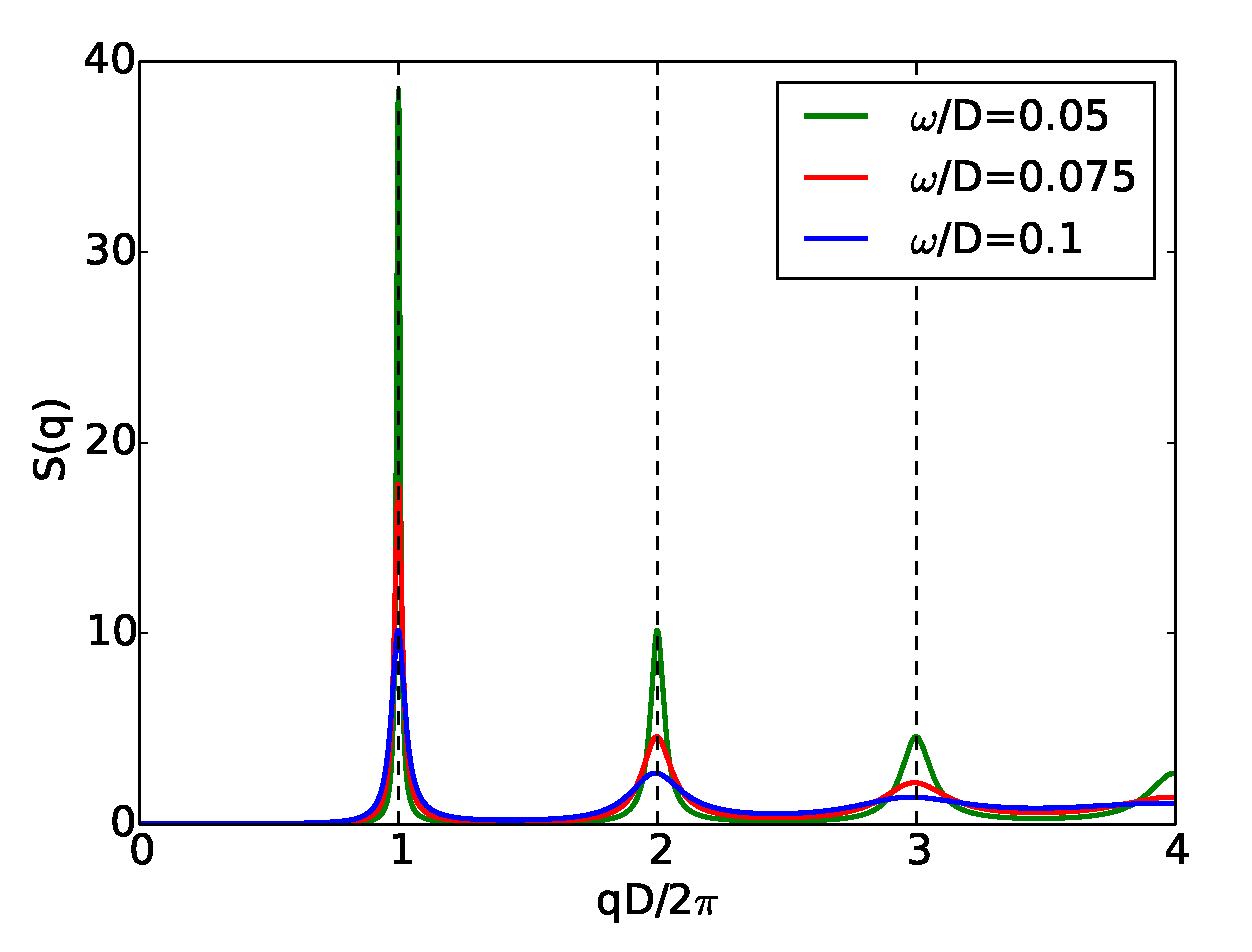
\includegraphics[width=0.6\textwidth]{fig/funcplot/S_q_1Dparacrystal.eps}
\end{center}
\caption{Interference function of a 1D Gaussian paracrystal plotted for different values of $\omega /D$. The peaks broaden with a decreasing amplitude as $\omega/D$ increases. This shows the transition between an ordered and a disordered states. }
\label{fig:1dparas_q}
\end{figure}

In two dimensions, the paracrystal is constructed on a pseudo-regular lattice with base vectors $\v{a}$ and $\v{b}$ using the following conditions for the densities of probabilities:

$\int p_{\v{a}}(\r)d^2r=\int p_{\v{b}}(\r)\d^2r=1$,
$\int \r p_{\v{a}}(\r)\d^2r=\v{a}$,
$\int \r p_{\v{b}}(\r)\d^2r=\v{b}$.

In the ideal case the deformations along the two axes are decoupled
and each unit cell should retain a parallelogram shape.
The interference function is given by
$S(q_{\plll})=\prod_{k=a,b}\Re\left(\dfrac{1+P_k(q_{\plll})}{1-P_k(q_{\plll})} \right)$
with $P_k$ the Fourier transform of $p_k$, $k=a, b$.

\paragraph{Probability distributions} \mbox{}\\
The scattering by an ordered lattice gives rise to a series of Bragg peaks situated at the nodes of the reciprocal lattice. Any divergence from the ideal crystalline case modifies the output spectrum by, for example, widening or attenuating the Bragg peaks. The influence of these "defects" can be accounted for
 in direct space by using correlation functions or by truncating the lattice or, in reciprocal space with structure factors or interference functions by convoluting the scattered peaks with a function which could reproduce the experimental shapes.

%===============================================================================
\subsection{Size-Spacing Correlation Approximation}
%===============================================================================
\index{Size-spacing correlation approximation}

TO MERGE IN:
introduces correlations between polydisperse particles, more precisely between the size of the particles and their mutual spacing. A classical example would consist in particles whose closest-neighbor spacing depends linearly on the sum of their respective sizes \cite{LaLR07}, as illustrated in \cref{fig:ssca}.

%For a sample where only the statistical properties of particle positions and size are known, the scattered intensity per scattering particle is expressed as the average over an ensemble of the Fourier transform of the Patterson function, which is the autocorrelation of the scattering length density $\curlp (\r ) \equiv \sum_{ij} S_i(-\r )\otimes S_j(\r )\otimes \delta (\r + \r_i - \r_j )$:
%\begin{equation*}
%  I(\q ) = \frac{1}{N}\ensavg{}{\curlf (\curlp (\r ))},
%\end{equation*}
%where $\curlf$ denotes the Fourier transform and $\curlp$ the Patterson function

\begin{figure}[tb]
\begin{center}
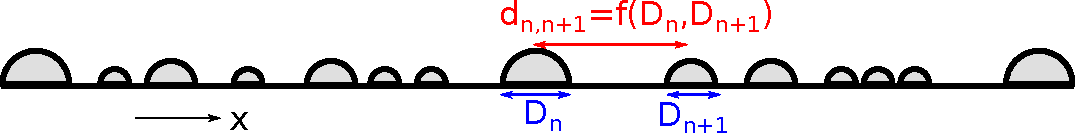
\includegraphics[width=0.9\textwidth]{fig/drawing/drawingSSCA.pdf}
\end{center}
\caption{Sketch of a 1D distributed collection of particles, whose scattering could be described by the size-spacing correlation approximation: the distance between two particles depends on their sizes.}
\label{fig:ssca}
\end{figure}


In the Size-Spacing Correlation Approximation, a correlation is assumed between the shape/size of the particles and their mutual spacing. A classical example would consist of particles whose closest-neighbor spacing depends linearly on the sum of their respective sizes. The following discussion of this type of correlation is inspired by \cite{LaLR07}

The scattered intensity can also be calculated as the Fourier transform of the Patterson function, which is the autocorrelation of the scattering length density:
\begin{equation*}
  \curlp (\r ) \equiv \sum_{ij} S_i(-\r )\otimes S_j(\r )\otimes \delta (\r + \r_i - \r_j ).
\end{equation*}
For a sample where only the statistical properties of particle positions and shape/size are known, the scattered intensity per scattering particle becomes average over an ensemble of the Fourier transform of the Patterson function:
\begin{equation*}
  I(\q ) = \frac{1}{N}\bra\curlf (\curlp (\r ))\ket,
\end{equation*}
where $\curlf$ denotes the Fourier transform.

The ensemble averaged Patterson function will be denoted as:
\begin{equation*}
  Z(r) \equiv \frac{1}{N}\bra\curlp (\r )\ket.
\end{equation*}
In the case of systems where the particles are aligned in one dimension, this autocorrelation function can be further split into nearest neighbor probabilities. First, it is split into terms for negative, zero or positive distance:
\begin{equation*}
  Z(\r ) \equiv z_0(\r ) + z_+(\r ) + z_-(\r ).
\end{equation*}
Taking $x$ as the coordinate in the direction in which the particles are arranged and $s$ as an orthogonal coordinate ($\r \equiv (x,s)$), one obtains:
\begin{align*}
  z_0(\r ) &= \sum_{\alpha_0} p(\alpha_0) S_{\alpha_0}(-x,-s) \otimes S_{\alpha_0}(x,s)  \\
  z_+(\r ) &= \sum_{\alpha_0\alpha_1} p(\alpha_0,\alpha_1) S_{\alpha_0}(-x,-s) \otimes S_{\alpha_1}(x,s) \otimes P_1(x|\alpha_0\alpha_1)  \\
               &+ \sum_{\alpha_0\alpha_1\alpha_2} p(\alpha_0,\alpha_1,\alpha_2) S_{\alpha_0}(-x,-s) \otimes S_{\alpha_2}(x,s) \otimes P_1(x|\alpha_0\alpha_1) \otimes P_2(x|\alpha_0\alpha_1\alpha_2)  \\
               &+ \dotsb \\
  z_-(\r ) &= z_+(-\r ),
\end{align*}
where $p(\alpha_0,\dotsc ,\alpha_n)$ denotes the probability of having a sequence of particles of the indicated sizes/shapes and $P_n(x|\alpha_0\dotsc\alpha_n)$ is the probability density of having a particle of type $\alpha_n$ at a (positive) distance $x$ of its nearest neighbor of type $\alpha_{n-1}$ in a sequence of the given order.

In the Size-Spacing Correlation Approximation, one assumes that the particle sequence probabilities are just a product of their individual fractions:
\begin{equation*}
  p(\alpha_0,\dotsc ,\alpha_n) = \prod_i p(\alpha_i),
\end{equation*}
and the nearest neighbor distance distribution is dependent only on the two particles involved:
\begin{equation*}
  P_n(x|\alpha_0\dotsc\alpha_n) = P_1(x|\alpha_{n-1}\alpha_n).
\end{equation*}
Furthermore, the distance distribution $P_1(x|\alpha_0\alpha_1)$ depends on the particle sizes/shapes only through its mean value $D$:
\begin{equation*}
  P_1(x|\alpha_0\alpha_1) = P_0(x - D(\alpha_0,\alpha_1) ),
\end{equation*}
where $D(\alpha_0,\alpha_1) = D_0 + \kappa \left[ \Delta R(\alpha_0) + \Delta R(\alpha_1) \right]$, with $\Delta R(\alpha_i)$ the deviation of a size parameter of particle $i$ with respect to the mean over all particles sizes/shapes and $\kappa$ the coupling parameter.

In momentum space, the sum of convolutions can be written as a geometric series, which can be exactly calculated to be:
\begin{equation}
\label{Esscainf}
I(\q ) = {\bra\left| F_\alpha(\q ) \right| ^2\ket}_{\alpha}
+ 2 \Re \left\lbrace \widetilde{\curlf_\kappa}(\q )
 \widetilde{\curlf_\kappa^*}(\q ) \cdot
 \frac{\Omega_\kappa(\q )}{\tilde{p}_{2\kappa}(\q )\left
   [ 1 - \Omega_\kappa(\q )\right] } \right\rbrace,
\end{equation}
with
\begin{align*}
  \tilde{p}_\kappa(\q ) &= \int \d\alpha\; p(\alpha) \e^{i\kappa q_x \Delta R(\alpha)}  \\
  \Omega_\kappa(\q ) &= \tilde{p}_{2\kappa}(\q ) \phi(\q) \e^{i q_x D_0}  \\
  \widetilde{\curlf_\kappa}(\q ) &=
       \int \d\alpha\; p(\alpha)F_\alpha (\q ) \e^{i\kappa q_x \Delta R(\alpha)},
\end{align*}
and the Fourier transform of $P_1(x|\alpha_0\alpha_1)$ is
\begin{equation*}
  \curlp (\q ) = \phi (\q )\e^{i q_x D_0}
                    \e^{i \kappa q_x \left[ \Delta R(\alpha_0) + \Delta R(\alpha_1) \right] }.
\end{equation*}

Using the result from the one-dimensional analysis, one can apply this formula ad hoc for distributions of particles in a plane, where the coordinate $x$ will now be replaced with $(x,y)$, while the $s$ coordinate encodes a position in the remaining orthogonal direction. One must be aware however that this constitutes a further approximation, since this type of correlation does not have a general solution in more than one dimension.

The intensity in \cref{Esscainf} will contain a Dirac delta function contribution, caused by taking an infinite sum of terms that are perfectly correlated at $\q = 0$. One can leverage this behaviour by multiplying the nearest neighbor distribution by a constant factor $\e^{-D/\Lambda}$, which removes the division by zero in \cref{Esscainf}.
Another way of dealing with this infinity at $\q =0$ consists of taking only a finite number of terms, in which case the geometric series still has an analytic solution, but becomes a bit more cumbersome:
\begin{equation*}
\begin{split}
  I(\q ) &= {\bra\left| F_\alpha(\q ) \right| ^2\ket}_\alpha
   + 2 \Re \Biggl\lbrace \frac{1}{\tilde{p}_{2\kappa}(\q )}\widetilde{\curlf_\kappa}(\q )\widetilde{\curlf_\kappa^*}(\q ) \\
  & \times \left[ \left( 1 - \frac{1}{N}\right) \frac{\Omega_\kappa(\q )}{1 - \Omega_\kappa(\q ) } - \frac{1}{N}\frac{\Omega_\kappa^2(\q )\left( 1- \Omega_\kappa^{N-1}(\q )\right) }{\left( 1 - \Omega_\kappa(\q ) \right) ^2 } \right] \Biggr\rbrace.
\end{split}
\end{equation*}
This expression has a well-defined limit for $\Omega_\kappa(\q ) \rightarrow 1$ (when $\q \rightarrow 0$), namely:
\begin{equation*}
  \lim_{\q \rightarrow 0} I(\q ) = {\bra\left| F_\alpha(0 ) \right| ^2\ket}_{\alpha} + \left( N-1 \right) \left| {\bra F_\alpha(0 )\ket}_{\alpha} \right|^2.
\end{equation*}


%%%%%%%%%%%%%%%%%%%%%%%%%%%%%%%%%%%%%%%%%%%%%%%%%%%%%%%%%%%%%%%%%%%%%%%%%%%%%%%%
\section{Vertical location of particles}
%%%%%%%%%%%%%%%%%%%%%%%%%%%%%%%%%%%%%%%%%%%%%%%%%%%%%%%%%%%%%%%%%%%%%%%%%%%%%%%%

 \Note{The particles cannot sit in between layers. At most they can be sitting on any inner interfaces.}

%===============================================================================
\subsection{Particles deposited on a substrate}
%===============================================================================
%Substrate modified Born approximation
In this configuration, the particles are sitting on top of a substrate layer, in the air as shown in \cref{fig:SchemDWBA}. In the DWBA the expression of a form factor becomes
\begin{align}
F_{\rm{DWBA}}(q_{\plll}, k_{i,z}, k_{f,z}) &= F_{\rm{BA}}(q_{\plll}, k_{i,z}-k_{f,z})+ R_i F_{\rm{BA}}(q_{\plll}, -k_{i,z}-k_{f,z}) \nonumber \\
&+ R_f F_{\rm{BA}}(q_{\plll}, k_{i,z}+k_{f,z}) + R_i R_f F_{\rm{BA}}(q_{\plll},-k_{i,z}+k_{f,z}), \label{Edwbaair}
\end{align}
where $q_{\plll}$ is the component of the scattering beam in the plane of the interface ($\q=\k_i-\k_\text{f}$), $k_{i,z}$ and $k_{f,z}$ are the z-component of the incident and scattered beam, respectively. $R_i$, $R_f$ are the reflection coefficients in incidence and reflection. They are defined as\\ $R=\dfrac{k_z+\sqrt{n_s^2k_0^2-|k_{\plll}|^2}}{k_z-\sqrt{n_s^2 k_0^2-|k_{\plll}|^2}}$, where $n_s=1-\delta_s +i \beta_s$ is the refractive index of the substrate, $k_0$ is the wavelength in vacuum ($2\pi /\lambda$), $k_z$ and $k_{\plll}$ are the $z$-component and the in-plane component of $\k_\text{i}$ or $\k_\text{f}$. \\

\Note{If the particles are sitting on a multilayered system, the expression of the form factor in the DWBA is obtained by replacing the Fresnel coefficient by the corresponding coefficients of the underlying layers \cite{Par54,BoWo99}.}

\vspace{18pt}

\Cref{fig:SchemDWBA} illustrates the four scattering processes for a supported particle, taken into account in the DWBA. The first term of eqn\.~\Cref{Edwbaair}  corresponds to the Born approximation. Each term of $F_{\rm{DWBA}}$ is weighted by a Fresnel coefficient.

\begin{figure}[tb]
\begin{center}
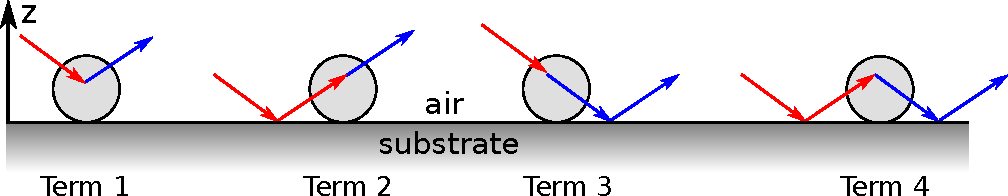
\includegraphics[width=\textwidth]{fig/drawing/drawingDWBA.pdf}
\end{center}
\caption{Schematic views of the different terms appearing in the expression of the form factor under DWBA for particles sitting on a substrate layer.}
\label{fig:SchemDWBA}
\end{figure}


Script~\ref{lst:badwba} illustrates the difference between BA and DWBA in \BornAgain\ when generating the sample.  We consider the simple case of:
\begin{itemize}
\item one kind of particles' shape,
\item no interference between the particles,
\item in the DWBA, a sample made of a layer of substrate on which are deposited the particles,
\item in the BA, a sample composed of the particles in air.
\end{itemize}

\Cref{fig:spheroidbadwba} shows the intensity contour plot generated using this script with truncated spheroids as particles.

\newpage

\begin{lstlisting}[language=python, style=eclipseboxed,numbers=none,nolol,caption={\Code{Python} script to generate a sample using Born (BA) or distorted-wave Born approximation (DWBA). The difference between BA and DWBA in this simple case is the absence or presence of a substrate layer in the sample.},label={lst:badwba}]
def get_sample():
    """
    Build and return the sample to calculate form factor of
    truncated spheroid in Born or distorted-wave Born Approximation.
    """
    # defining materials
    m_ambience = HomogeneousMaterial("Air", 0.0, 0.0)
    m_substrate = HomogeneousMaterial("Substrate", 6e-6, 2e-8)
    m_particle = HomogeneousMaterial("Particle", 6e-4, 2e-8)

    # collection of particles
    ff= FormFactorTruncatedSpheroid(7.5*nanometer, 9.0*nanometer, 1.2)
    particleshape = Particle(m_particle, ff)
    particle_layout = ParticleLayout()
    particle_layout.addParticle(particleshape, 1.0)

    # interferences
    interference = InterferenceFunctionNone()
    particle_layout.addInterferenceFunction(interference)

    # assembling the sample
    air_layer = Layer(m_ambience)
    air_layer.addLayout(particle_layout)
    substrate_layer = Layer(m_substrate, 0)

    multi_layer = MultiLayer()
    multi_layer.addLayer(air_layer)
    # Comment the following line out for Born Approximation
    multi_layer.addLayer(substrate_layer)
    return multi_layer
\end{lstlisting}


\begin{figure}[tb]
\hfill
\subfigure[Born Approximation]{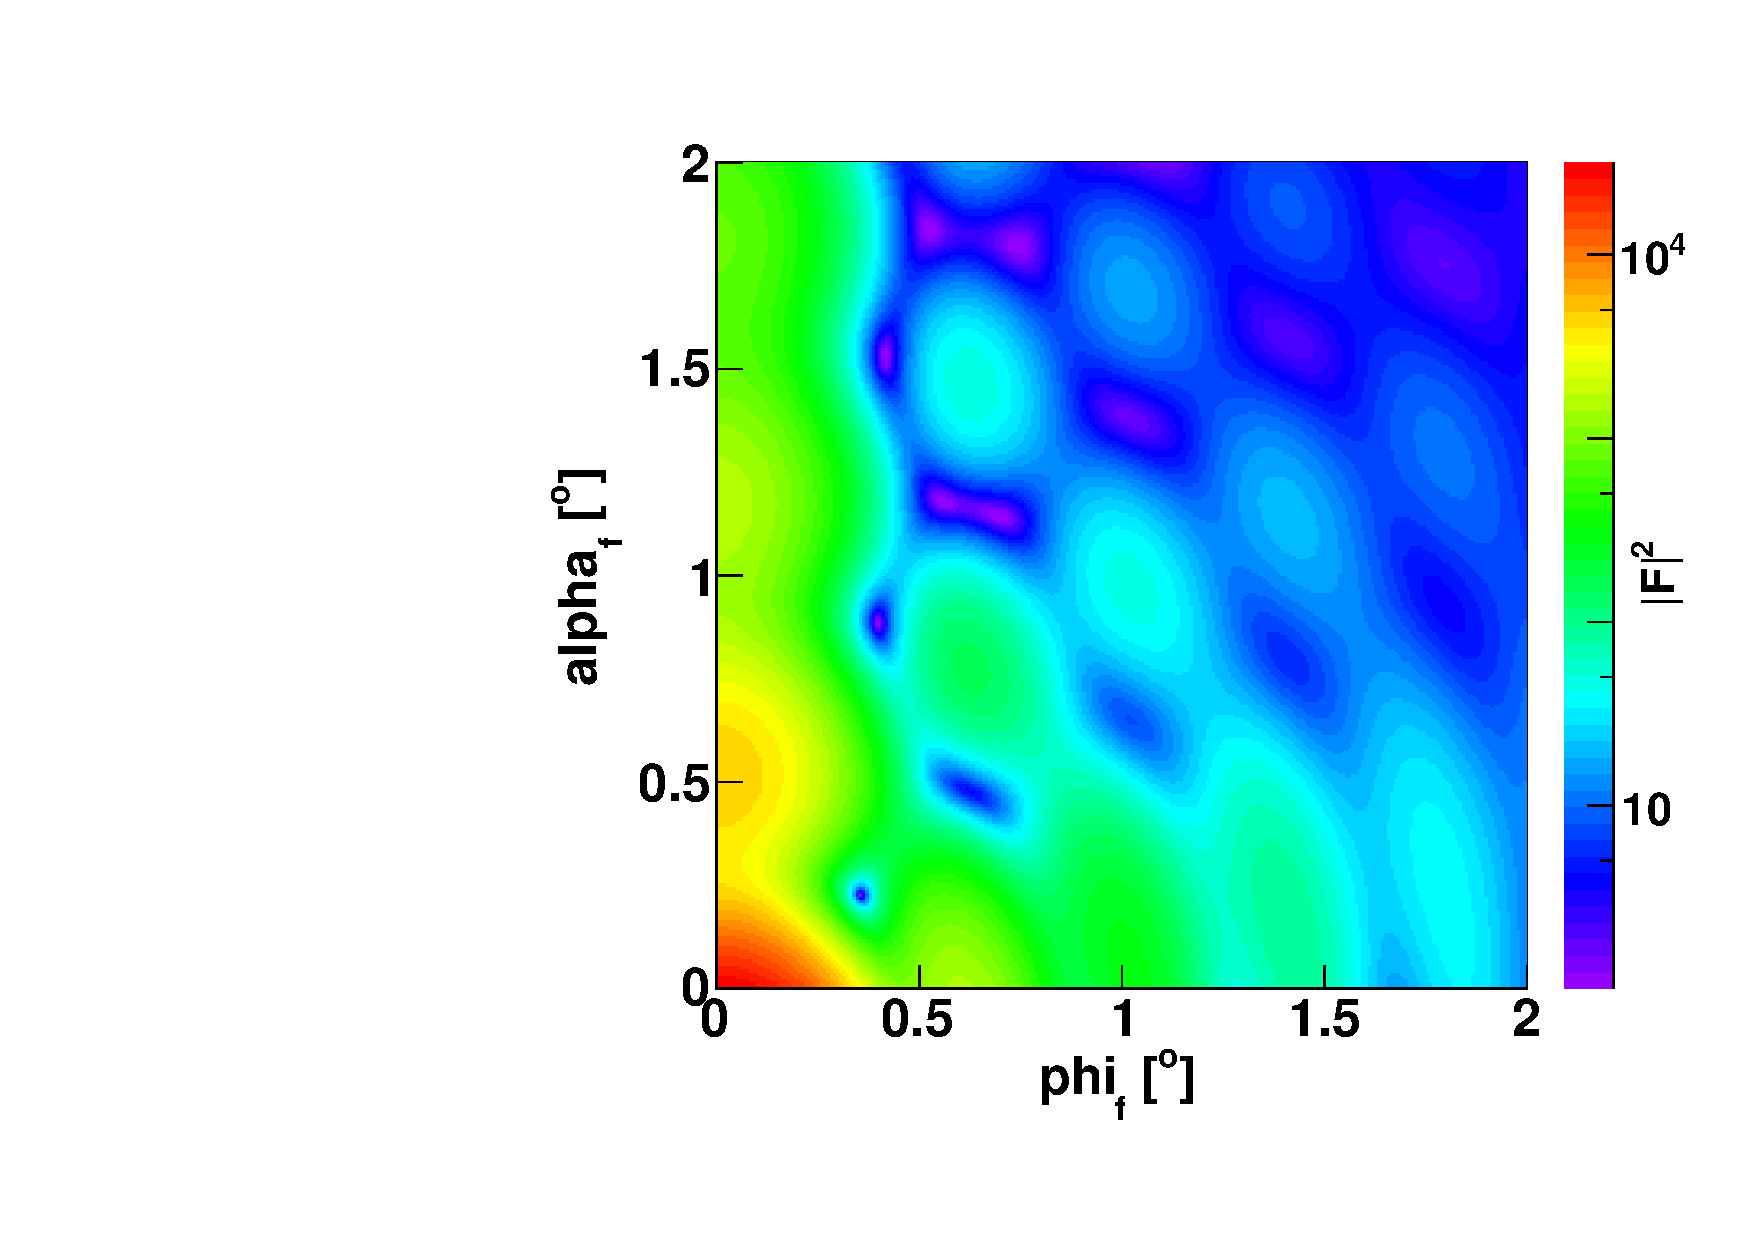
\includegraphics[angle=-90,width=6cm]{fig/gisasmap/ffspheroidBA.pdf}}
\hfill
\subfigure[DWB Approximation]{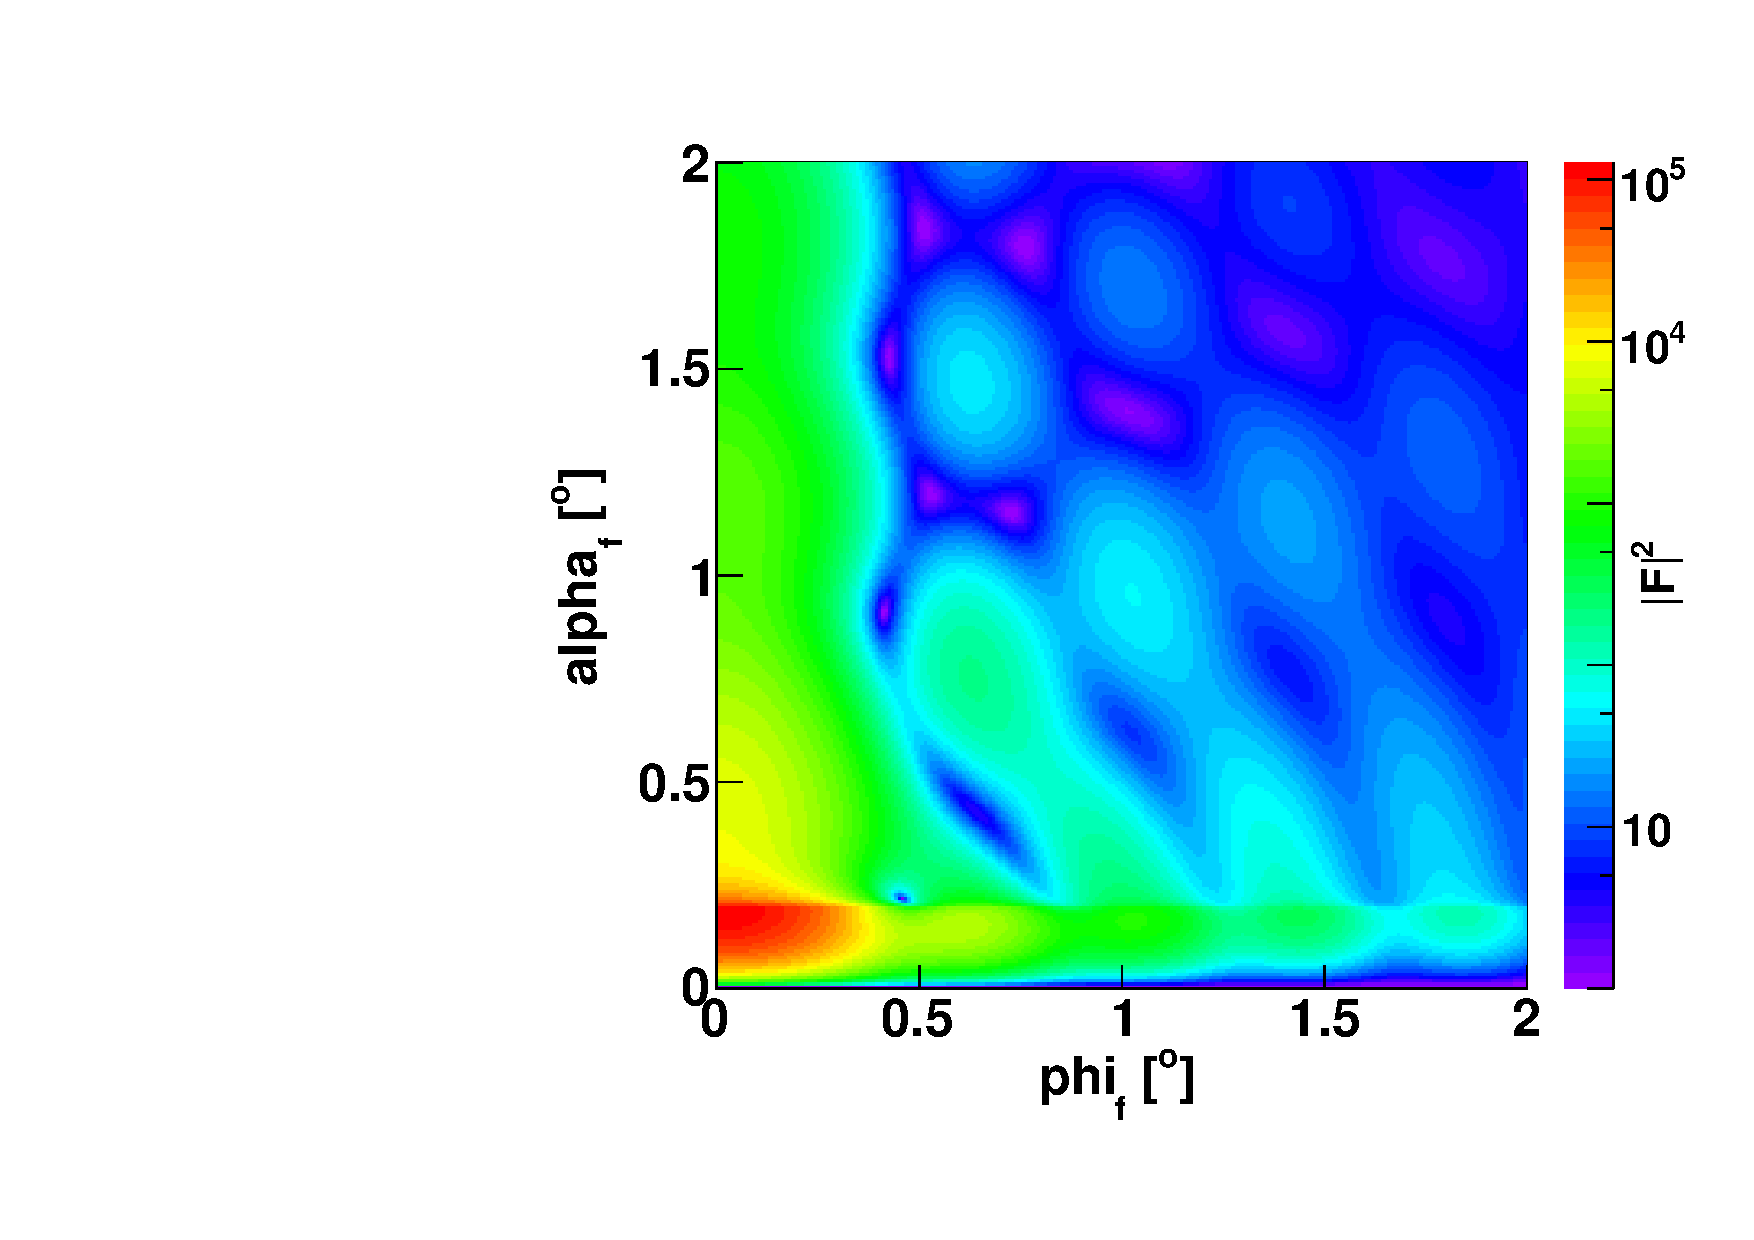
\includegraphics[angle=-90,width=6cm]{fig/gisasmap/ffspheroidDWBA.pdf}}
\hfill
\caption{Intensity map of TruncatedSpheroid form factor in BA and DWBA computing using script~\ref{lst:badwba} for the sample.}
\label{fig:spheroidbadwba}
\end{figure}

\FloatBarrier

\Note{In \BornAgain, the DWBA is implemented automatically when assembling the sample with more layers than only the air layer (for example, for particles are sitting on a substrate).}

%===============================================================================
\subsection{Buried particles}
%===============================================================================

The system considered in this section consists of particles encapsulated in a layer, which is sitting on a substrate (see \cref{fig:SchemDWBAburied}). In this case the form factor in the DWBA is given by

\begin{align}
  F_{\rm{DWBA}}(q_{\plll}, k_{i,z}, k_{f,z})
  &= T_\text{i} T_\text{f} F_{\rm{BA}}(q_{\plll}, k_{i,z}-k_{f,z})\e^{i(k_{i,z}-k_{f,z})d}\nonumber \\
  &+ R_\text{i} T_\text{f} F_{\rm{BA}}(q_{\plll}, -k_{i,z}-k_{f,z})\e^{i(-k_{i,z}-k_{f,z})d} \nonumber \\
  &+ R_\text{f} T_\text{i} F_{\rm{BA}}(q_{\plll}, k_{i,z}+k_{f,z}) \e^{i(k_{i,z}+k_{f,z})d}\nonumber \\
  &+ R_\text{f} R_\text{i}F_{\rm{BA}}(q_{\plll},-k_{i,z}+k_{f,z})\e^{i(-k_{i,z}+k_{f,z})d}, \label{Edwbaburied}
\end{align}

\begin{equation*}
R_j =\frac{t^{j}_{0,1}r^{j}_{1,2}\exp(2ik_{j,z}t)}{1+r^{j}_{0,1}r^{j}_{1,2}\exp(2ik_{j,z}t)}, \quad T_j=\frac{t^{j}_{0,1}}{1+r^{j}_{0,1}r^{j}_{1,2}\exp(2ik_{j,z}t)}, j=i,f
\end{equation*}
where $q_{\plll}$ is the component of the scattering beam in the plane of the interface, $k_{i,z}$ and $k_{f,z}$ are the z-component of the incident and scattered beams, respectively.  $d$ is the depth at which the particles are sitting in the layer. Note that this value is given relative to the top of this layer and it is not the coordinate in the absolute referential (linked with the full sample) and it is measured up to the bottom of the particle. $t$ is the thickness of the intermediate layer containing the particles. $R_{i,f}$ and $T_{i,f}$  are the reflection  and transmission coefficients in incidence and reflection (they can be calculated using Parratt or matrix formalism). $r^j_{0,1}$, $r^j_{1,2}$ $t^j_{0,1}$ are the reflection and transmission coefficients between layers; the indices are related to different boundaries with 0: air, 1: intermediate layer and 2: substrate layer and the superscript $j$ is associated with the incident or scattered beams:
\begin{equation*}
r^j_{n,n+1}=\frac{k_{j,z,n}-k_{j,z,n+1}}{k_{j,z,n}-k_{j,z,n+1}}, \qquad t^j_{n,n+1}= \frac{2k_{j,z,n}}{k_{j,z,n}-k_{j,z,n+1}}, \quad n=0,1, \quad j=i,f,
\end{equation*}
where index $n$ is related to the layers, $z$ to the vertical component, and $j$ to the beams (incident and outgoing).

\begin{figure}[tb]
\begin{center}
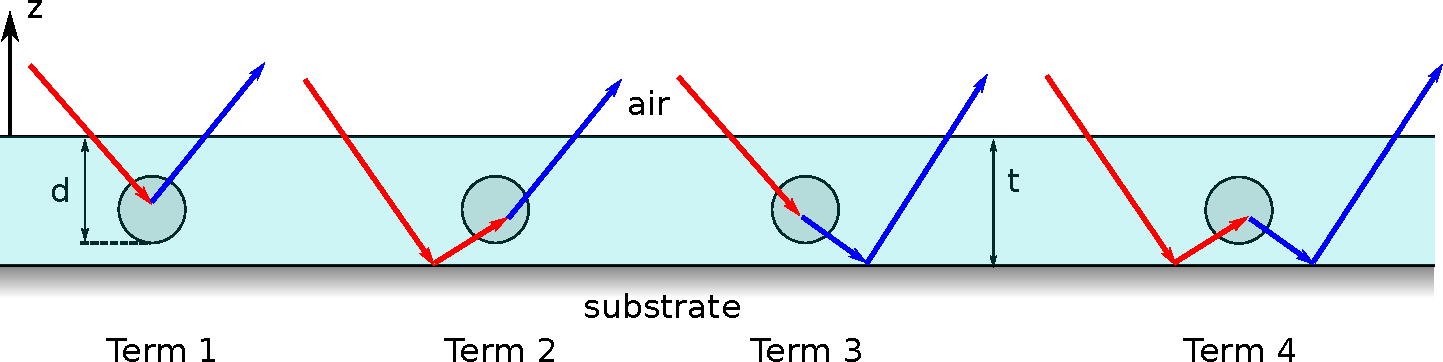
\includegraphics[width=\textwidth]{fig/drawing/drawingDWBAburied.pdf}
\end{center}
\caption{Schematic views of the different terms appearing in the expression of the form factor under the DWBA for buried particles.}
\label{fig:SchemDWBAburied}
\end{figure}


\Cref{fig:dwbaburied} shows a typical example of the output intensity scattered from a sample made of 3 layers: air, substrate, and in between, spherical particles embedded in the middle of a 30~nm-thick layer. This figure had been generated using listing~\ref{lst:dwbaburied}.

\begin{lstlisting}[language=python, style=eclipseboxed,numbers=none,nolol,caption={\Code{Python} script to generate a sample where spherical particles are embedded in the middle of a layer on a substrate.},label={lst:dwbaburied}]
def get_sample():
    """
    Build and return the sample with buried spheres in DWBA.
    """
    # defining materials
    m_ambience = HomogeneousMaterial("Air", 0.0, 0.0)
    m_interm_layer = HomogeneousMaterial("IntermLayer",3.45e-6, 5.24e-9)
    m_substrate = HomogeneousMaterial("Substrate", 7.43e-6, 1.72e-7)
    m_particle = HomogeneousMaterial("Particle", 0.0, 0.0)

    # collection of particles
    ff = FormFactorFullSphere(10.2*nanometer)
    particleshape = Particle(m_particle, ff)
    particleshape.setPosition(0.0, 0.0, -25.2)
    particle_layout = ParticleLayout()
    particle_layout.addParticle(particleshape, 1.0)

    # interferences
    interference = InterferenceFunctionNone()
    particle_layout.addInterferenceFunction(interference)

    # assembling the sample
    air_layer = Layer(m_ambience)
    intermediate_layer = Layer(m_interm_layer, 30.*nanometer)
    intermediate_layer.addLayout(particle_layout)
    substrate_layer = Layer(m_substrate, 0)

    multi_layer = MultiLayer()
    multi_layer.addLayer(air_layer)
    multi_layer.addLayer(intermediate_layer)
    multi_layer.addLayer(substrate_layer)
    return multi_layer
\end{lstlisting}


\begin{figure}[tb]
\centering
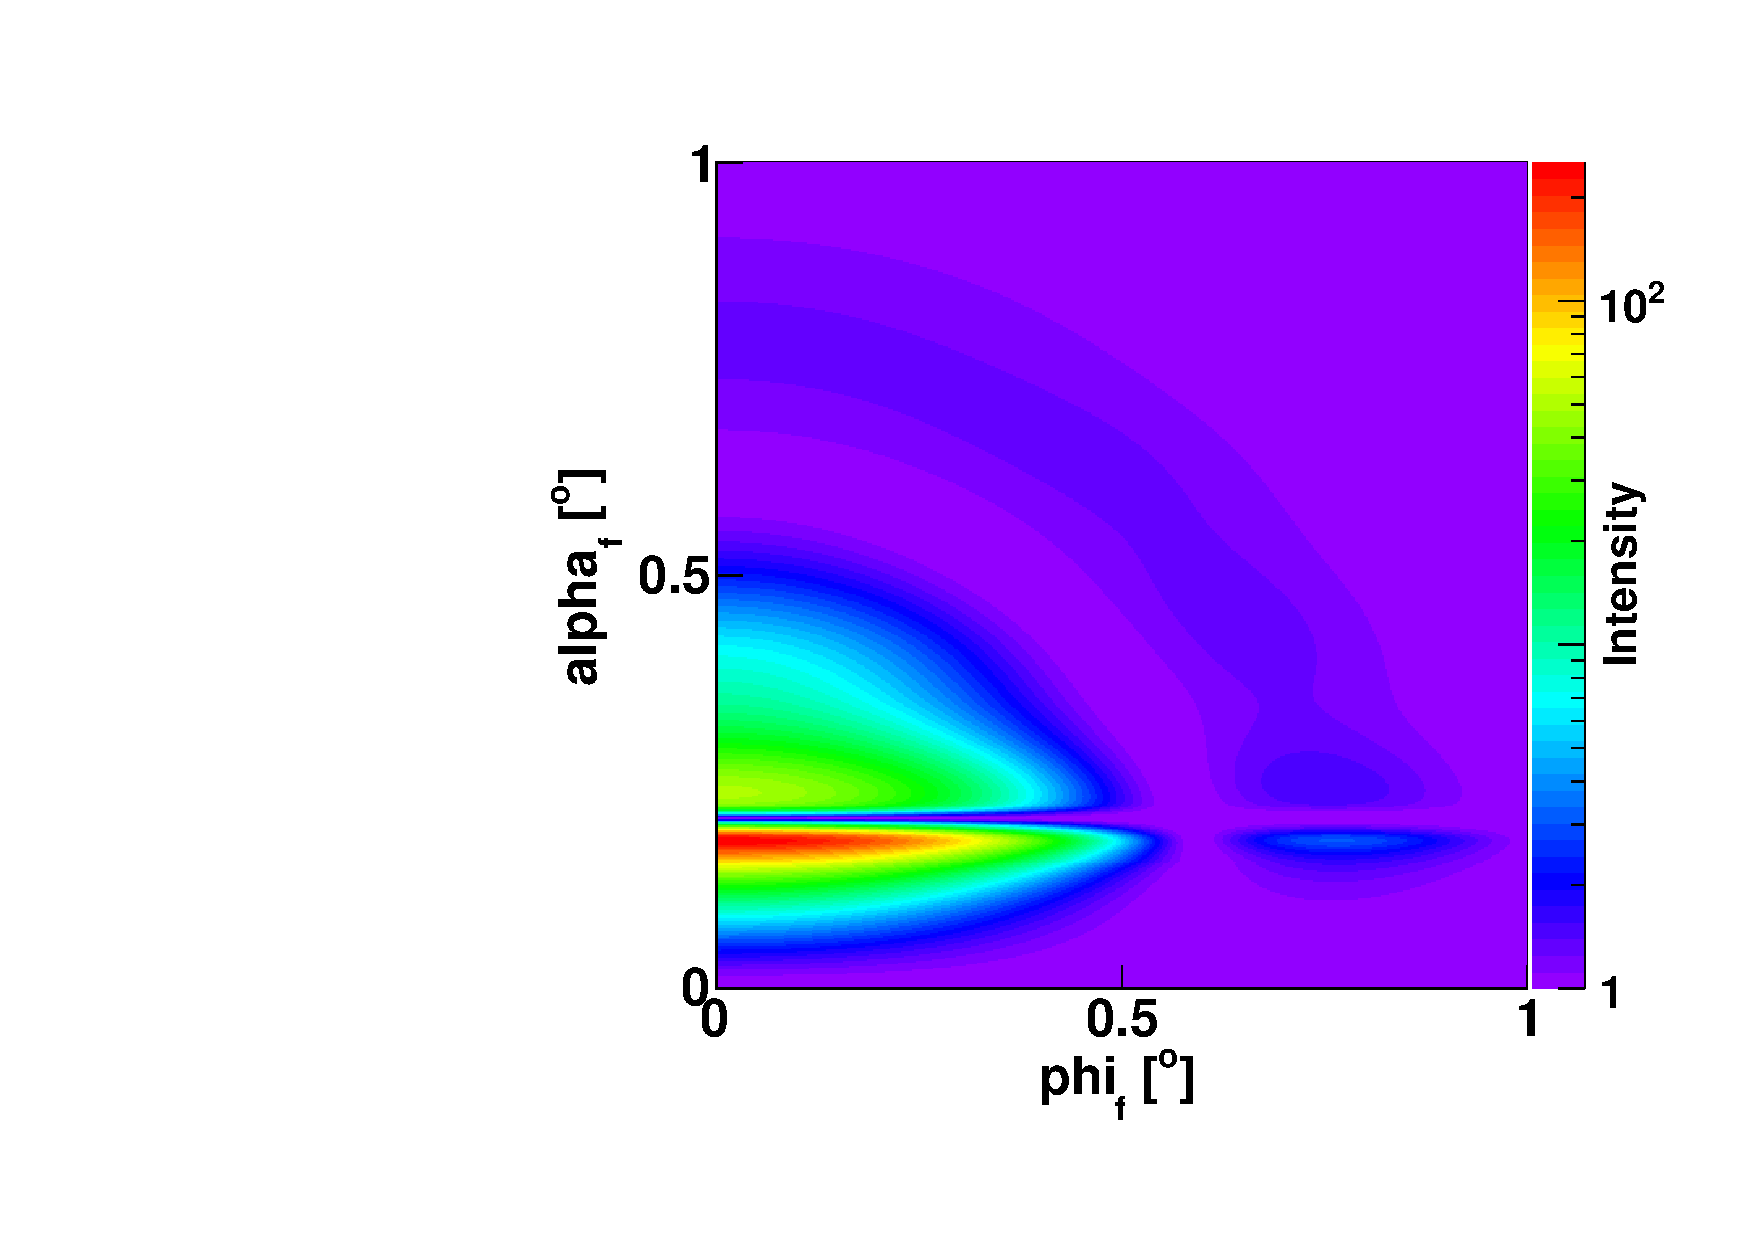
\includegraphics[angle=-90,width=0.6\textwidth]{fig/gisasmap/figIntBuriedPart.pdf}
\caption{Map of intensity scattered from a sample made of spherical particles embedded in the middle of a 30~nm-thick layer on a substrate (see Script~\ref{lst:dwbaburied} for details about the sample).}
\label{fig:dwbaburied}
\end{figure}

\newpage

\Note{For layers different from the air layer, the top interface is considered as the reference level to position the encapsulated particles. For example, spheres positioned at depth $d$ (positive) are located at a distance $d$ from the top of the layer up to the bottom of these particles. This convention is different for the top air layer, where particles sitting at the interface with an underlying layer (\idest the bottom of the air layer) are located at depth 0 (see \cref{fig:depthpartBA}).}


\begin{figure}[tb]
\centering
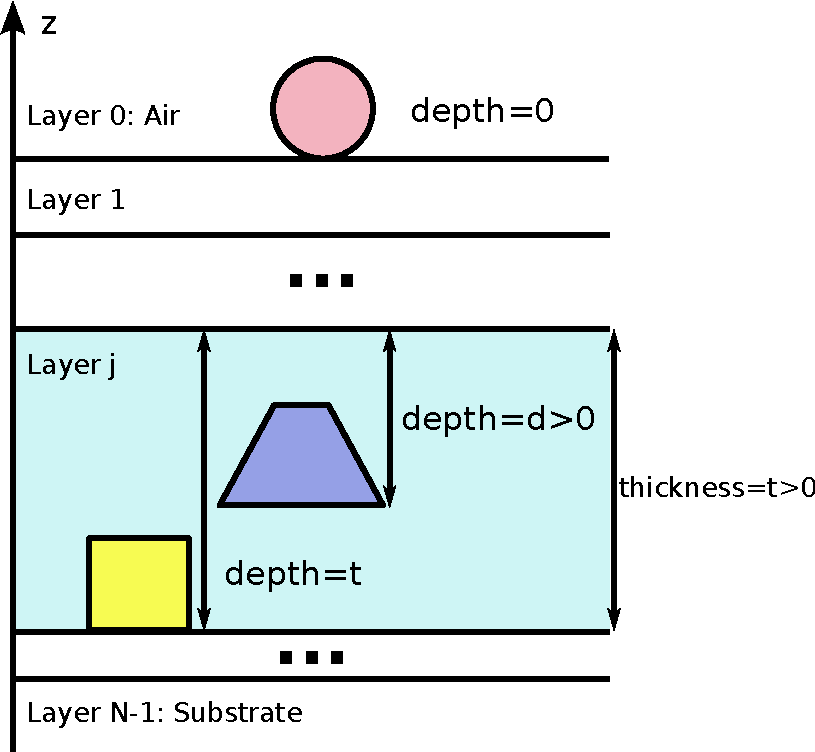
\includegraphics[width=0.5\textwidth]{fig/drawing/drawingDepthParticle.pdf}
\caption{Illustration of the convention about \Code{depth} used in \BornAgain\ to encapsulate particles in layers.}
\label{fig:depthpartBA}
\end{figure}


%%%%%%%%%%%%%%%%%%%%%%%%%%%%%%%%%%%%%%%%%%%%%%%%%%%%%%%%%%%%%%%%%%%%%%%%%%%%%%%%
\section{Implementation in \BornAgain}
%%%%%%%%%%%%%%%%%%%%%%%%%%%%%%%%%%%%%%%%%%%%%%%%%%%%%%%%%%%%%%%%%%%%%%%%%%%%%%%%

This section describes the implementation of the interference functions in \BornAgain.
For an implementation of all the components of a simulation,
the use is referred, for example, to \cref{sec:Example1Python}.\\


\Note{In \BornAgain\ the particles are positioned in the same vertical layer.}

\subsection{Size-distribution models}
\index{Size-distribution models}
The decoupling approximation (DA), local monodisperse approximation (LMA) and size spacing correlation approximation (SSCA) can be used in \BornAgain.
The selection between DA and SSCA is made using\\
\Code{ILayout.setApproximation(EInterferenceFunction approximation)} when defining the characteristics of the way particles and interference functions are embedded in a layer.  For example,
\begin{lstlisting}[language=python, style=eclipseboxed,numbers=none,nolol]
    particle_layout = ParticleLayout()
   ....
# interference approx chosen between: DA (default) and SSCA
    particle_layout.setApproximation(ILayout.DA)
\end{lstlisting}

Note that with the SSCA, the users have to specify the coupling parameter $\kappa$ (with the function \Code{setKappa}), which should be a positive dimensionless value. $\kappa$ characterizes the influence of the neighboring particles' sizes on their distance. If $\kappa=0$, the SSCA reduces to the DA with a radial paracrystal for the interference function.\\

For the LMA, its implementation is automatically done when using more than one layout of particles:
\begin{lstlisting}[language=python, style=eclipseboxed,numbers=none,nolol]
    particle_layout0 = ParticleLayout()
    particle_layout1 = ParticleLayout()
   ....
# association of each particles' layout with materials, form factors
#... and with a material layer
    layer_a = Layer(m_material_a)
    layer_a.addLayout(particle_layout0)
    layer_a.addLayout(particle_layout1)
\end{lstlisting}

%%ADD EXPLANATION ABOUT LMA

%-------------------------------------------------------------------------------
\subsection{Probability distribution functions}\label{baftd}
%-------------------------------------------------------------------------------

The probability distribution functions have been implemented in the reciprocal space in \BornAgain. Their expressions are given in Table~\ref{table:pdf}.

\begin{table}[H]
\centering
\begin{tabular}{ccc}
\hline
Function & One dimension & Two dimensions\\
\hline
Cauchy & $(1+q^2\omega^2)^{-3/2}$ & $(1 + q_x^2 cl_x^2 + q_y^2 cl_y^2)^{-3/2}$ \\
Gauss & $\dfrac{1}{2}\exp(-\dfrac{q^2\omega^2}{4})$ & $\frac{1}{2}\exp\left(-\dfrac{q_x^2 cl_x^2+ q_y^2cl_y^2}{4}\right)$ \\
Voigt & $\dfrac{\eta}{2} \exp\left(-\dfrac{q^2\omega^2}{4}\right) + \dfrac{1 - \eta}{(1 + q^2\omega^2)^{3/2}}$ & $\dfrac{\eta}{2} \exp\left(-\dfrac{q_x^2 cl_x^2+ q_y^2cl_y^2}{4}\right)+ \dfrac{1 - \eta}{(1 + q_x^2 cl_x^2+ q_y^2cl_y^2)^{3/2}}$ \\
\hline
\end{tabular}
\caption{List of probability distribution functions in reciprocal space. $\omega$, $cl$ stand for coherence lengths (the index refers to the axis) and  $\eta$ is a weighting coefficient.}
\label{table:pdf}
\end{table}

The Cauchy distribution corresponds to $\exp(-r)$ in real space and the Voigt one  is a linear combination of the Gaussian and Cauchy probability distribution functions.\\

\noindent \underline{One dimension}
\begin{itemize}
\item \Code{FTDistribution1DCauchy($\omega$)},
\item \Code{FTDistribution1DGauss($\omega$)},
\item \Code{FTDistribution1DVoigt($\omega, \eta$)}.
\end{itemize}
where $\omega$ is the coherence length and $\eta$ is a weighting factor.\\

\noindent \underline{Two dimensions}
\begin{itemize}
\item \Code{FTDistribution2DCauchy($cl_x$, $cl_y$)},
\item \Code{FTDistribution2DGauss($cl_x$, $cl_y$)},
\item \Code{FTDistribution2DVoigt($cl_x$, $cl_y$)}
\end{itemize}
where $cl_{x,y}$ are the coherence lengths in the $x$ or $y$ direction, respectively.

These functions can be used with all interference functions, except the case without any interference.

%-------------------------------------------------------------------------------
\subsection{Interferences}
%-------------------------------------------------------------------------------
\index{Interference function}

The interference function is specified when building the sample. It is linked with the particles (shape, material). Examples of implementation are given at the end of each description.

\paragraph{Syntax:}
 \Code{particle\_layout.addInterferenceFunction(interference\_function)},\\ where \Code{particle\_layout} holds the information about the different shapes and their proportions for a given layer of particles, and \Code{interference\_function}  is one of the following expressions:
\begin{itemize}
\item \Code{InterferenceFunctionNone()}
\item \Code{InterferenceFunction1DLattice(lattice\_parameters)}
\item \Code{InterferenceFunctionRadialParaCrystal(peak\_distance, damping\_length)}
\item \Code{InterferenceFunction2DLattice(lattice\_parameters)}
\item \Code{InterferenceFunction2DParaCrystal(length\_1, length\_2, $\alpha$\_lattice, $\xi$, \\ damping\_length)}
\end{itemize}

\Note{\Code{InterferenceFunction1DLattice} can only be used for particles which are infinitely long in one direction of the sample's surface like for example a rectangular grating.}

\newpage
%-------------------------------------------------------------------------------
\subsection{InterferenceFunctionNone}
%-------------------------------------------------------------------------------

The particles are placed randomly in the dilute limit and are considered as individual, non-interacting scatterers. The scattered intensity is function of the form factors only.

\paragraph{Example} The sample is made of a substrate on which are deposited half-spheres. Script~\ref{lst:nointerf} details the commands necessary to generate such a sample. \Cref{fig:nointerf} shows an example of output intensity: Script~\ref{lst:nointerf}  + detector's + input beam's characterizations.


\begin{figure}[tb]
\begin{center}
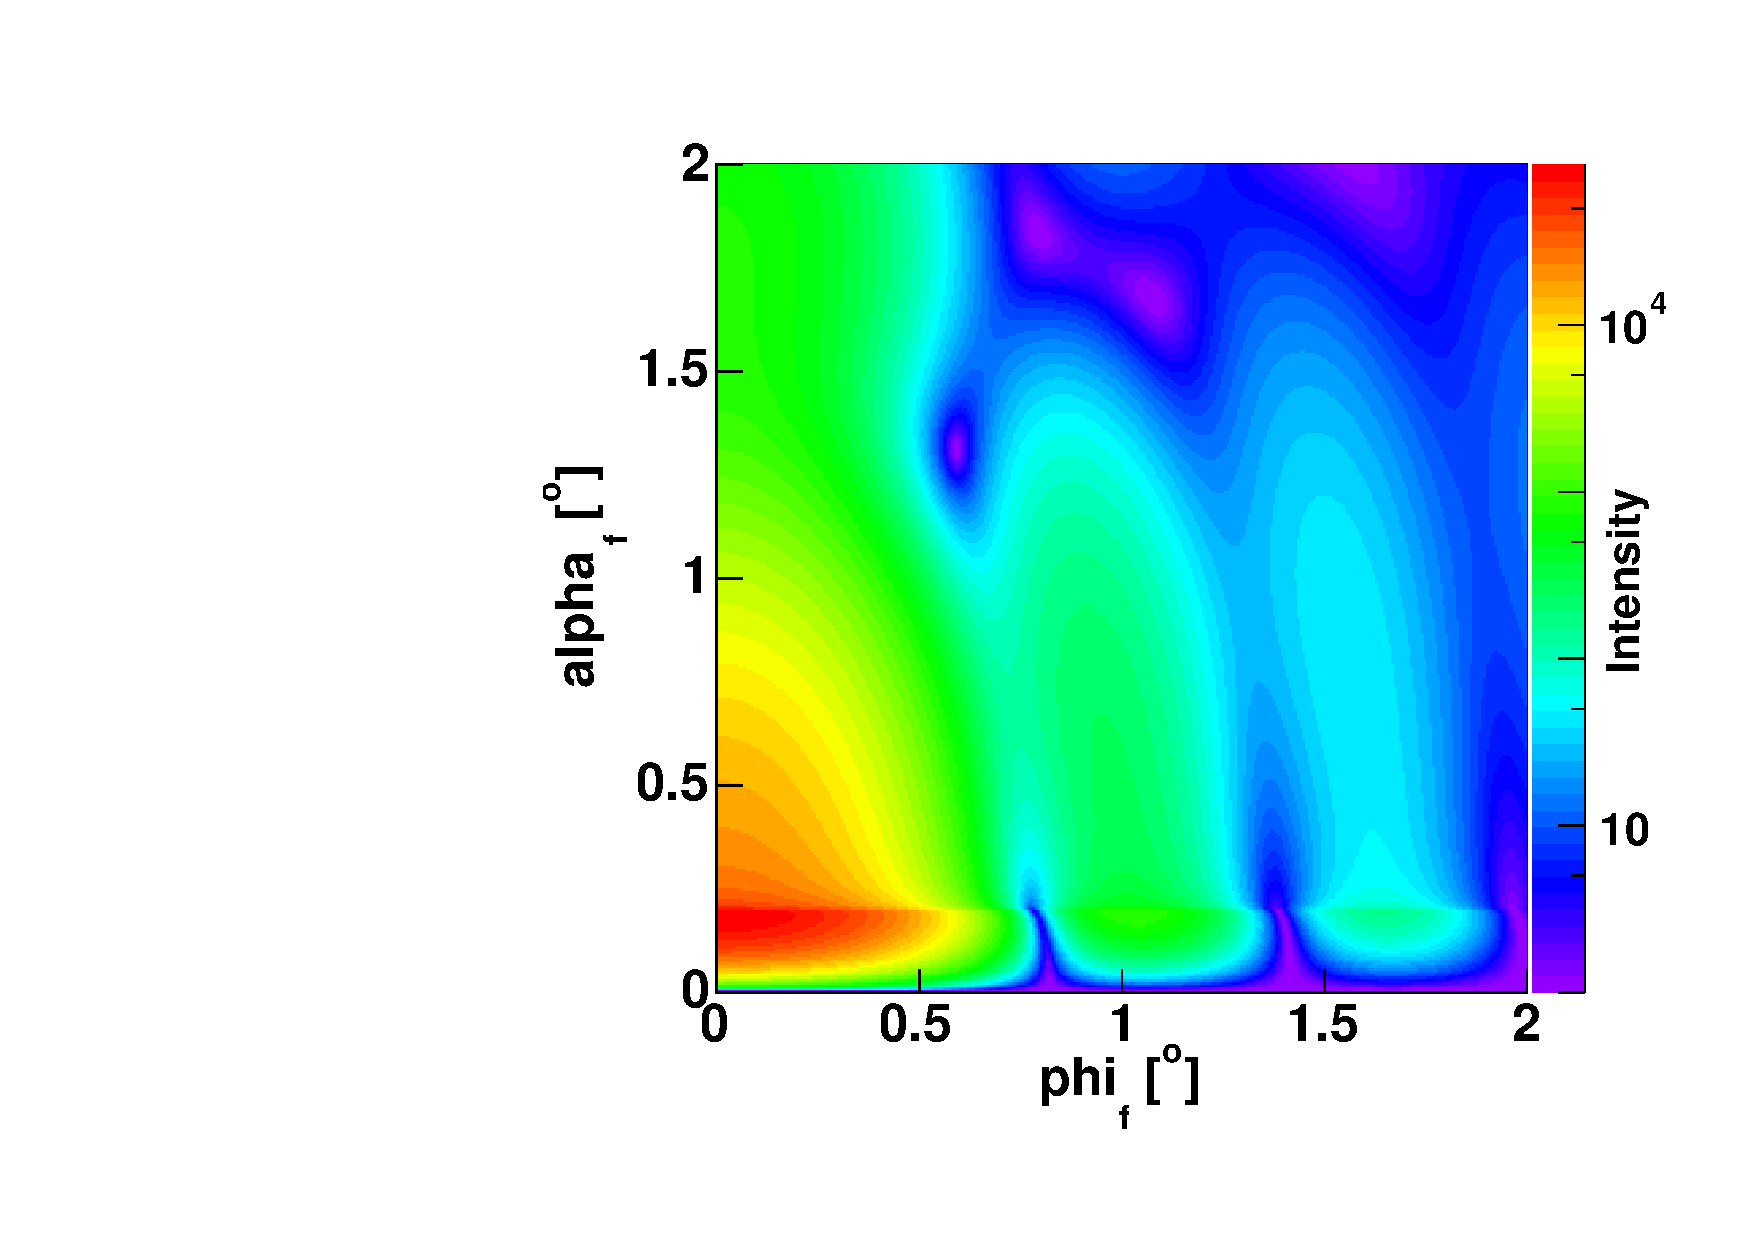
\includegraphics[angle=-90,width=0.5\textwidth]{fig/gisasmap/HSphere_NoInterf.pdf}
\end{center}
\caption{Output intensity scattered from a sample made of half-spheres with no interference between them.}
\label{fig:nointerf}
\end{figure}

\FloatBarrier
\newpage

\begin{lstlisting}[language=python, style=eclipseboxed,numbers=none,nolol,caption={\Code{Python} script to simulate a sample made of half-spheres deposited on a substrate layer without any interference. The part specific to the interferences is marked in a red italic font.},label={lst:nointerf}]
def get_sample():
    """
    Build and return the sample representing particles with no interference
    """
    # defining materials
    m_ambience = HomogeneousMaterial("Air", 0.0, 0.0)
    m_substrate = HomogeneousMaterial("Substrate", 6e-6, 2e-8)
    m_particle = HomogeneousMaterial("Particle", 6e-4, 2e-8)
    # collection of particles
    sphere_ff = FormFactorTruncatedSphere(5*nanometer, 5*nanometer)
    sphere = Particle(m_particle, sphere_ff)
    particle_layout = ParticleLayout()
    particle_layout.addParticle(sphere, 1.0)
    |interference = InterferenceFunctionNone()|
    |particle_layout.addInterferenceFunction(interference)|
    # assembling the sample
    air_layer = Layer(m_ambience)
    air_layer.addLayout(particle_layout)
    substrate_layer = Layer(m_substrate, 0)

    multi_layer = MultiLayer()
    multi_layer.addLayer(air_layer)
    multi_layer.addLayer(substrate_layer)
    return multi_layer
\end{lstlisting}

\newpage
%-------------------------------------------------------------------------------
\subsection{\Code{InterferenceFunction1DLattice(lattice\_length, xi)}}
%-------------------------------------------------------------------------------
where lattice\_length is the lattice constant and $\xi$ the angle in radian between the lattice unit vector and the $\v{x}$-axis of the reference Cartesian frame as shown in \cref{fig:1dgrating}.

\begin{figure}[tb]
\begin{center}
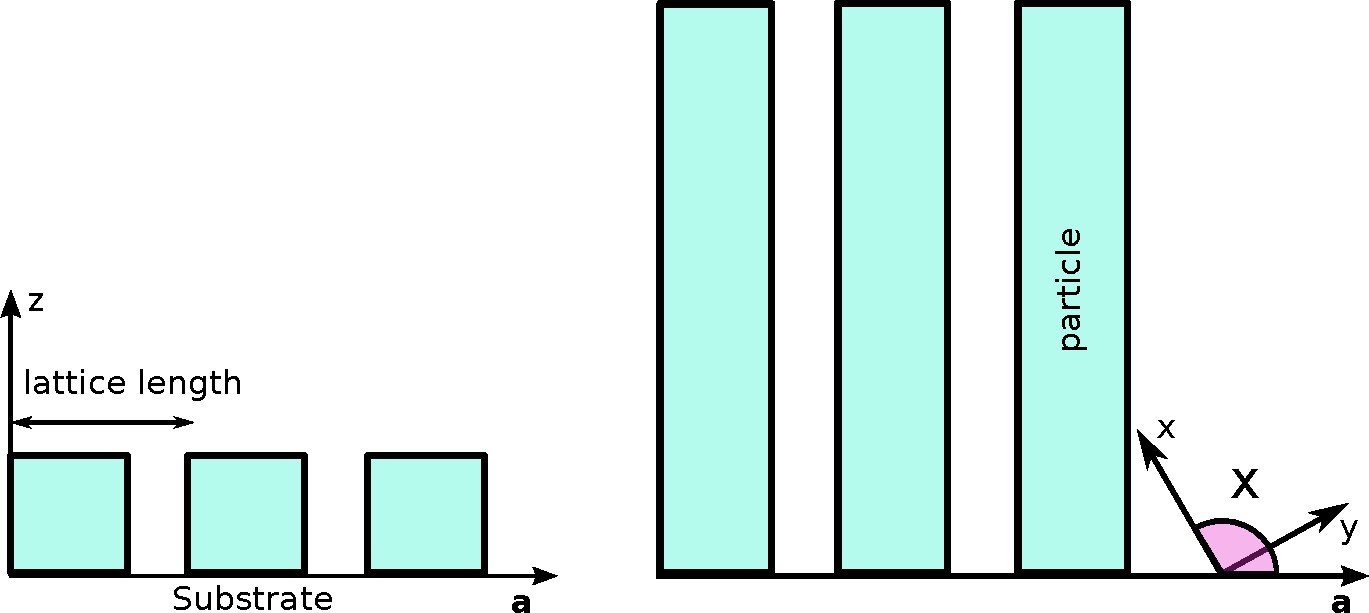
\includegraphics[width=0.75\textwidth]{fig/drawing/1DGrating.pdf}
\end{center}
\caption{Schematic representation of a 1D lattice (side and top views). Such a lattice is characterized by a lattice length and the angle $\xi$.}
\label{fig:1dgrating}
\end{figure}

\Note{By default the long axis of the particles in this 1D lattice is along the beam axis. That is the reason why in the example below the particles are rotated by  $90^{\circ}$ in the $(x,y)$ plane: the main axis of the lattice is therefore parallel to the y-axis, perpendicular to the long axis of the particles.}

\vspace{12pt}
A probability distribution function \Code{pdf} has to be chosen from the list in \cref{baftd} in order to apply some modifications to the scattering peaks. This function is implemented using \Code{setProbabilityDistribution(pdf)}.

\paragraph{Example:} Script~\ref{lst:1dlattinterf} details how to build in  \BornAgain\ a sample using\\ \Code{InterferenceFunction1DLattice} as the interference function. As mentioned previously, this interference function can only be used with infinitely wide or long particles.\\ Here the sample is made of infinitely long boxes deposited on a substrate (these particles are characterized by their widths and heights). They are also rotated by $90^{\circ}$  in the sample surface in order to have their long axis perpendicular to the input beam, which is along the $x$-axis.\\
 The lattice parameters (the lattice length and angle between the lattice main axis and the $x$-axis) are passed into the constructor of the interference function.

\newpage
\begin{lstlisting}[language=python, style=eclipseboxed,numbers=none,nolol,caption={\Code{Python} script to generate a sample made of infinitely long boxes deposited on a substrate layer with the 1DLatticeInterference function. The part specific to the interferences is marked in a red italic font.},label={lst:1dlattinterf}]
def get_sample():
    """
    Build and return the sample with 1DLatticeInterference function
    """
    # defining materials
    m_air = HomogeneousMaterial("Air", 0.0, 0.0)
    m_substrate = HomogeneousMaterial("Substrate", 6e-6, 2e-8)
    m_particle = HomogeneousMaterial("Particle", 6e-4, 2e-8)

    # collection of particles
    ff = FormFactorInfLongBox(10.*nanometer, 15.0*nanometer)
    box = Particle(m_particle, ff)
    particle_layout = ParticleLayout()
    transform = Transform3D.createRotateZ(90.0*degree)
    particle_layout.addParticle(box, transform)

    # interference function
    |interference = InterferenceFunction1DLattice(30.0*nanometer, 0.0*degree)|
    |pdf = FTDistribution1DCauchy(200./2./M_PI*nanometer)|
    |interference.setProbabilityDistribution(pdf)|
    |particle_layout.addInterferenceFunction(interference)|

    # air layer with particles and substrate form multi layer
    air_layer = Layer(m_air)
    air_layer.addLayout(particle_layout)
    substrate_layer = Layer(m_substrate, 0)

    multi_layer = MultiLayer()
    multi_layer.addLayer(air_layer)
    multi_layer.addLayer(substrate_layer)
    return multi_layer
\end{lstlisting}

\newpage
%-------------------------------------------------------------------------------
\subsection{\Code{InterferenceFunctionRadialParaCrystal(peak\_distance, damping\_length)}}
%-------------------------------------------------------------------------------
\begin{itemize}
\item[where] \Code{peak\_distance} is the average distance to the first neighbor peak,
\item[]\Code{width} is the width parameter of the probability distribution,
\item[] \Code{damping\_length} is used to introduce finite size effects by applying a multiplicative coefficient equal to  $\exp$(-\Code{peak\_distance/damping\_length}) to the Fourier transform of the probability densities. \Code{damping\_length} is equal to 0 by default and, in this case, no correction is applied.
\end{itemize}

A probability distribution function \Code{pdf} has to be chosen from the list in \cref{baftd} in order to apply some modifications to the scattering peaks. This function is implemented using \Code{setProbabilityDistribution(pdf)}.


\Note{
This interference function is not one-dimensional.  It takes into account the radial component of the scattering vector.
}

\paragraph{Example}
To illustrate the radial paracrystal interference function, we use the same sample as in the case without interference: half-spheres deposited on a substrate.

\begin{lstlisting}[language=python, style=eclipseboxed,numbers=none,nolol,caption={\Code{Python} script to define the radial paracrystal interference function between half-spheres, where \Code{trsphere} is of type \Code{Particle}.},label={lst:1dpara}]
    particle_layout = ParticleLayout()
    particle_layout.addParticle(trsphere, 1.0)
    interference = InterferenceFunctionRadialParaCrystal(25.0*nanometer, 1e3*nanometer)
    pdf = FTDistribution1DGauss(7 * nanometer)
    interference.setProbabilityDistribution(pdf)
    particle_layout.addInterferenceFunction(interference)
\end{lstlisting}



\begin{figure}[tb]
\begin{center}
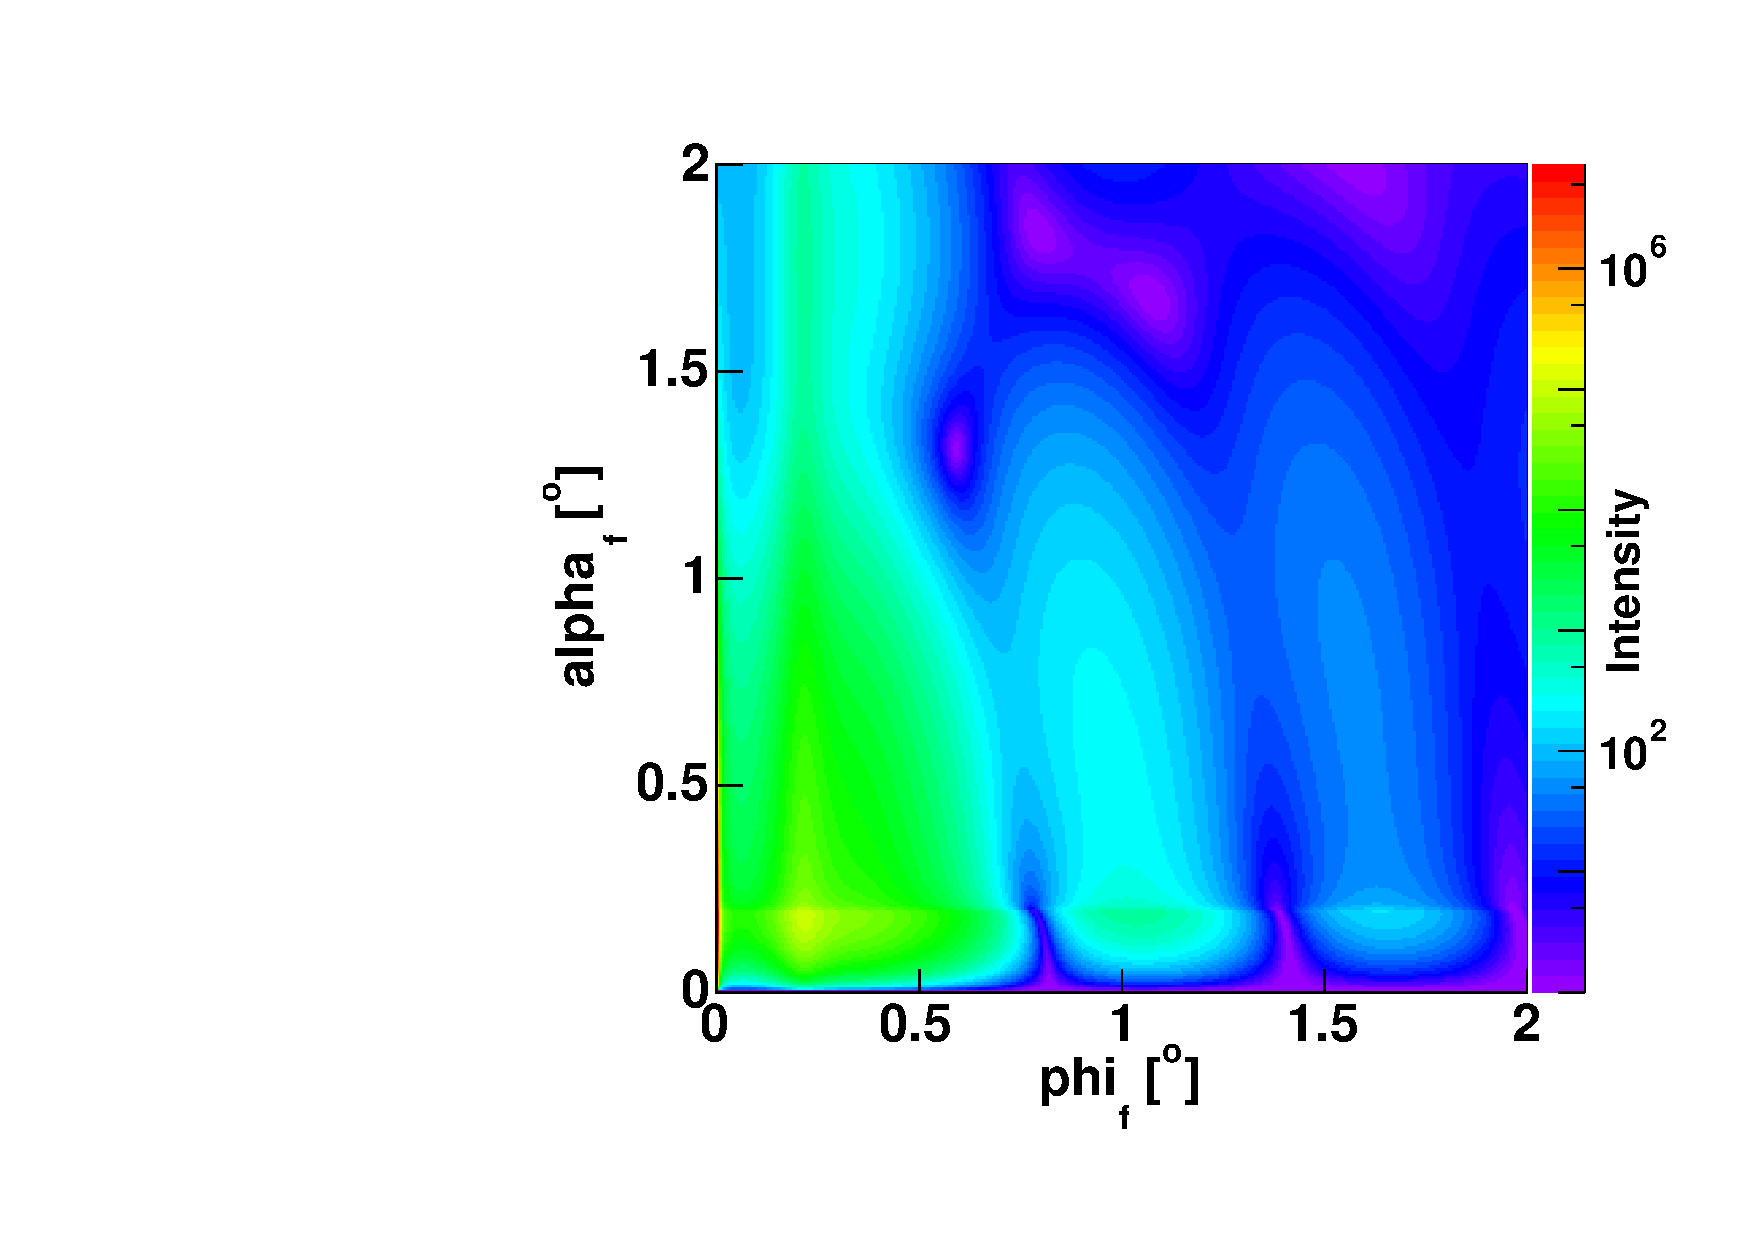
\includegraphics[angle=-90,width=0.5\textwidth]{fig/gisasmap/HSphere_1DDL.pdf}
\end{center}
\caption{Output intensity scattered from a sample made of half-spheres with the radial paracrystal interference between them. This figure has been generated using Script~\ref{lst:1dpara} for the interference function.}
\label{fig:1ddl}
\end{figure}

\FloatBarrier

\newpage
%-------------------------------------------------------------------------------
\subsection{\Code{InterferenceFunction2DLattice(L\_1, L\_2, alpha, xi)}}
%-------------------------------------------------------------------------------
where ($L_1$, $L_2$, $\alpha$, $\xi$) are shown in \cref{fig:2dlattice} with
\begin{itemize}
\item[]$L_1$, $L_2$ the lengths of the lattice cell,
\item[]$\alpha$ the angle between the lattice basis vectors $\v{a}, \v{b}$ in direct space,
\item[] $\xi$ is the angle defining the lattice orientation (set to $0$ by default); it is taken as the angle between the $\v{a}$ vector of the lattice basis and the $\v{x}$ axis of the reference Cartesian frame (as shown in \cref{fig:multil3d}).
\end{itemize}

\begin{figure}[tb]
\begin{center}
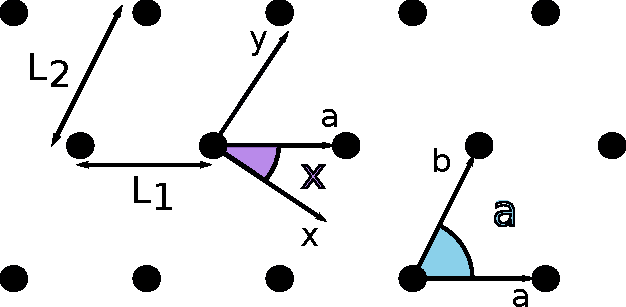
\includegraphics[width=0.5\textwidth]{fig/drawing/2Dlattice.pdf}
\end{center}
\caption{Schematic representation of a 2D lattice (top view). Such a lattice is characterized by lattice lengths $L_1$, $L_2$ and angles $\alpha$ and $\xi$.}
\label{fig:2dlattice}
\end{figure}

Like for the one-dimensional case, a probability distribution function \Code{pdf} has to be defined. One can choose between those listed in \cref{baftd} and implements it using \Code{setProbabilityDistribution(pdf)}.

\paragraph{Example} The sample used to run the simulation is made of half-spheres deposited on a substrate. The interference function is "2Dlattice" and the particles are located at the nodes of a square lattice with $L_1=L_2=20$~nm, $\v{a}\equiv \v{b}$ and the probability distribution function is Gaussian. We also use the Decoupling Approximation.

\begin{lstlisting}[language=python, style=eclipseboxed,numbers=none,nolol,caption={\Code{Python} script to define a 2DLattice interference function between hemi-spherical particles as well as the Decoupling Approximation in \Code{getSimulation()}.  The part specific to the interferences is marked in a red italic font.},label={lst:2dlatticeinterf}]
    #collection of particles
    sphere_ff = FormFactorTruncatedSphere(5*nanometer, 5*nanometer)
    sphere = Particle(m_particle, sphere_ff)
    |interference = InterferenceFunction2DLattice(20.0*nanometer, 20.0*nanometer, 90.0*degree, 0.0*degree)|
    |pdf = FTDistribution2DGauss(200.0*nanometer/2.0/M_PI, 75.0*nanometer/2.0/M_PI)|
    |interference.setProbabilityDistribution(pdf)|
    particle_layout = ParticleLayout()
    particle_layout.addParticle(sphere, 1.0)
    |particle_layout.addInterferenceFunction(interference)|

    # interference approx chosen between: DA (default) and SSCA
    |particle_layout.setApproximation(ILayout.DA)|
\end{lstlisting}

%\begin{lstlisting}[language=python, style=eclipseboxed,numbers=none,nolol]
%def get_simulation():
%    """
%    Create and return GISAXS simulation with beam and detector
%    """
%    simulation = Simulation()
%    simulation.setDetectorParameters(100, 0.0*degree, 2.0*degree, 100, 0.0*degree, 2.0*degree, True)
%    simulation.setBeamParameters(1.0*angstrom, 0.2*degree, 0.0*degree)
%    return simulation
%\end{lstlisting}


\begin{figure}[tb]
\begin{center}
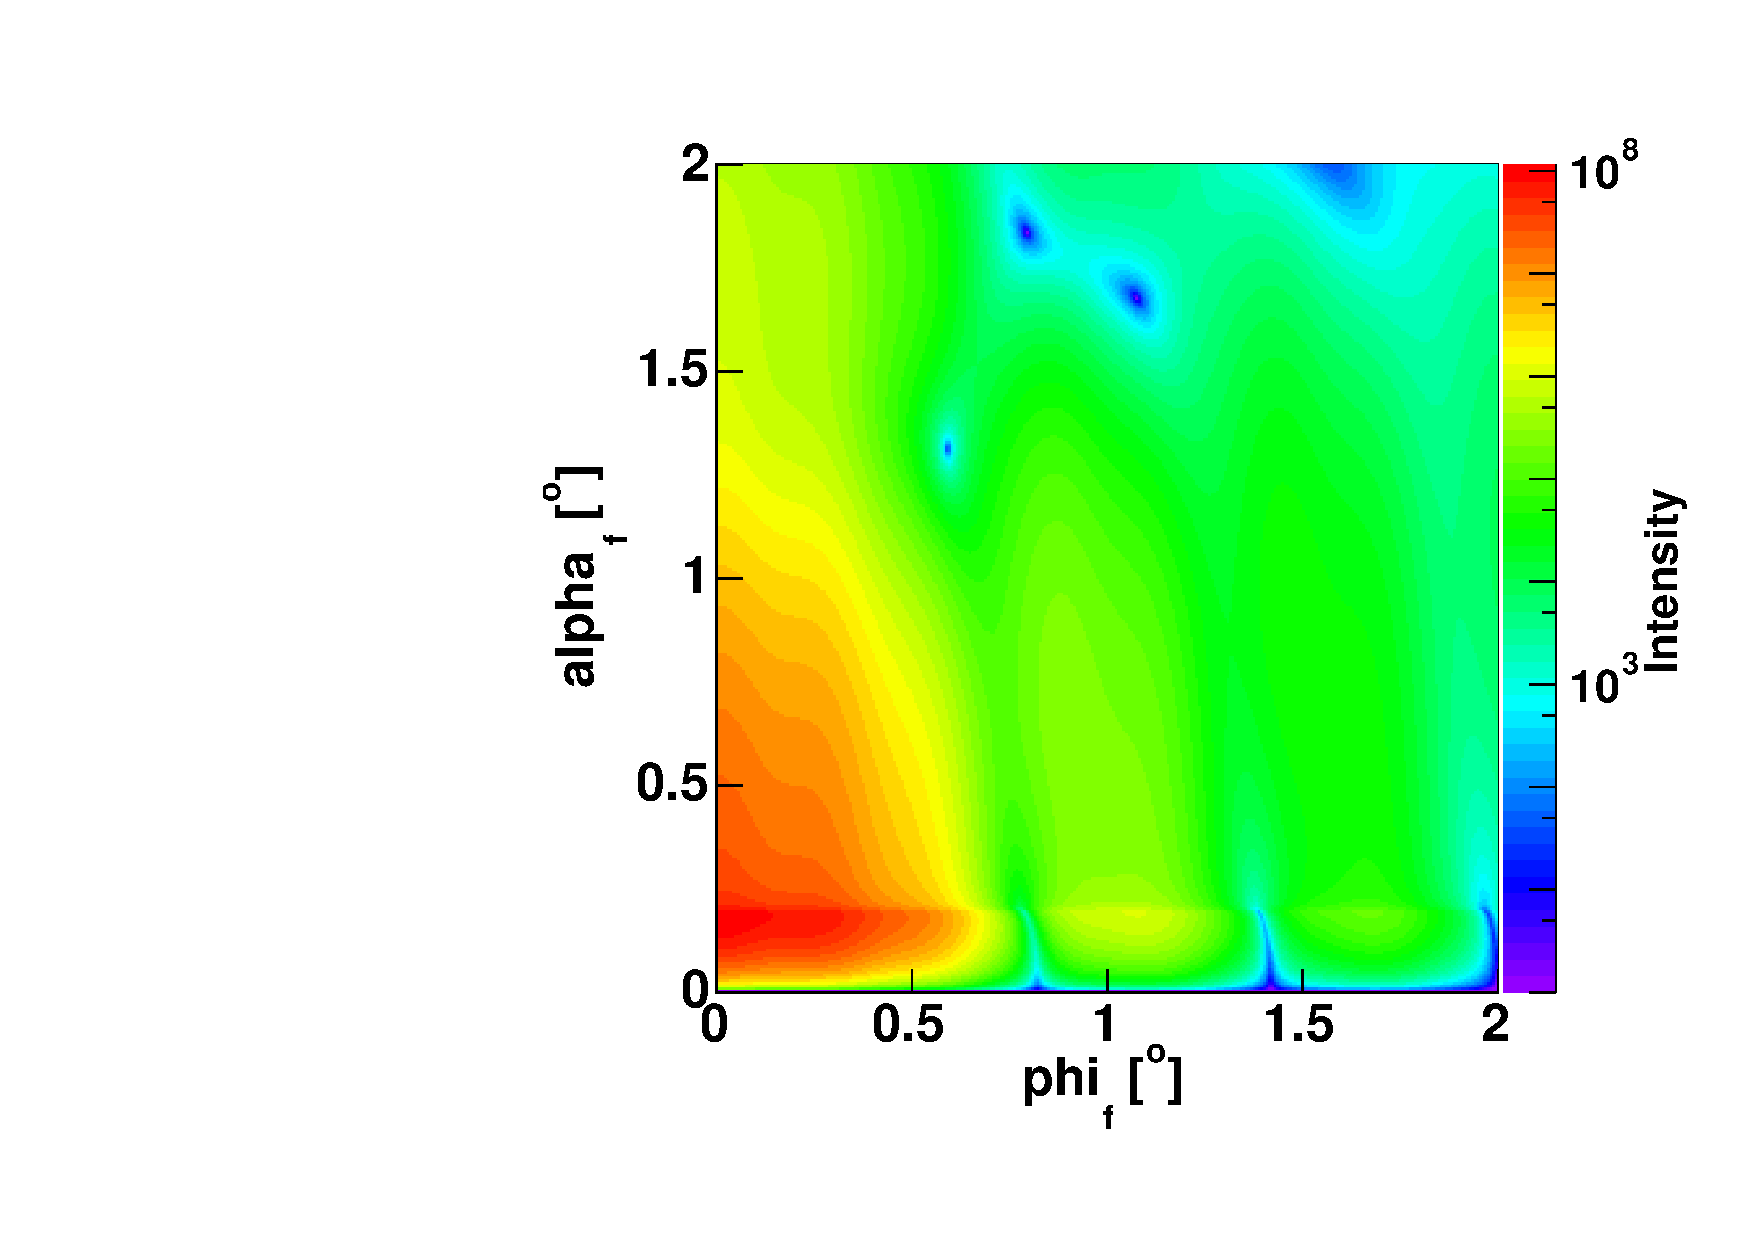
\includegraphics[angle=-90,width=0.5\textwidth]{fig/gisasmap/HSphere_2Dlattice.pdf}
\end{center}
\caption{Output intensity scattered from a sample made of half-spheres with 2DLattice interference function in the Decoupling Approximation.}
\label{fig:2dlatticeintensity}
\end{figure}

\FloatBarrier

\newpage%{\cleardoublepage}
%-------------------------------------------------------------------------------
\subsection{InterferenceFunction2DParaCrystal($L_1$, $L_2$, lattice\_angle, $xi$, damping\_length)} % TODO RESTORE \Code{}, \xi
%-------------------------------------------------------------------------------
\begin{itemize}
\item[where] $L_1$, $L_2$ are the lengths of the lattice cell,
\item[] lattice\_angle the angle between the lattice basis vectors $\v{a}, \v{b}$ in direct space,
\item[] $\xi$ is the angle defining the lattice orientation (set to $0$ by default).
\item[] \Code{damping\_length} is used to introduce finite size effects by applying a multiplicative coefficient equal to  $\exp$(-\Code{peak\_distance/damping\_length}) to the Fourier transform of the probability densities. \Code{damping\_length} is equal to 0 by default and, in this case, no correction is applied.
\end{itemize}
Two predefined interference functions can also be used:
\begin{itemize}
\item  \Code{createSquare(peak\_distance, damping\_length, domain\_size\_1, domain\_size\_2)}\\
where the angle between the base vectors of the lattice is set to $\pi/2$,
it creates a squared lattice,
\item \Code{createHexagonal(peak\_distance, damping\_length, domain\_size\_1, domain\_size\_2)}\\
where the angle between the base vectors of the lattice is set to $2\pi/3$ ,
\end{itemize}
where
\Code{domain\_size1, 2} are the dimensions of coherent domains of the paracrystal along the main axes,\\ \Code{peak\_distance} is the same in both directions and $\v{a}\equiv \v{x}$.\\

Probability distribution functions have to be defined. As the two-dimensional paracrystal is defined from two independent one-dimensional paracrystals, we need two of these functions, using\\ \Code{setProbabilityDistributions(pdf\_1, pdf\_2)}, with \Code{pdf\_{1,2}} related to each main axis of the paracrystal (see \cref{fig:2dparaschematic}).


\begin{figure}[tb]
\begin{center}
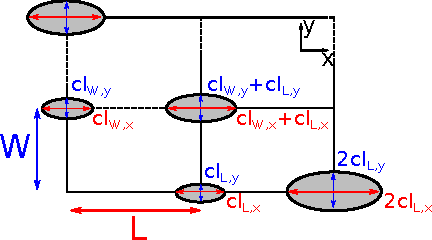
\includegraphics[width=0.75\textwidth]{fig/drawing/drawing2Dparacrystal.pdf}
\end{center}
\caption{Schematics of the ideal 2D paracrystal. The gray-shaded areas mark the regions where the probability to find a node is larger that the width at half-maximum of the distribution. $L$ and  $W$ are the mean inter-node distances along the two crystallographic axes. cl$_{(L,W),(x,y)}$ are the widths of the distribution of distance. The disorder is propagated as we add more nodes. Such a structure would be generated using \Code{InterferenceFunction2DParacrystal(L,W,90.*degrees,0,damp\_length)}, with \Code{pdf$_1$ = FTDistribution2DGauss(cl$_{L,x}$,cl$_{L,y}$)} and  \Code{pdf$_2$ = FTDistribution2DGauss(cl$_{W,x}$,cl$_{W,y}$)}.}
\label{fig:2dparaschematic}
\end{figure}


\paragraph{Example} The particles deposited on a substrate are half-spheres. The scattered beams interference via the 2DParacrystal distribution function. The paracrystal is based on a 2D hexagonal lattice with a Gaussian probability distribution function in reciprocal space.  Script~\ref{lst:2dparainterf} shows the implementation of the interference function and \cref{fig:2ddl} an example of output intensity using hemi-spherical particles.

\begin{lstlisting}[language=python, style=eclipseboxed,numbers=none,nolol,caption={\Code{Python} script to define a "2DParacrystal" interference function between particles forming an hexagonal monolayer. },label={lst:2dparainterf}]
    interference = InterferenceFunction2DParaCrystal.createHexagonal(30.0*nanometer,0.0, 40.0*micrometer, 40.0*micrometer)|
    pdf = FTDistribution2DCauchy(1.0*nanometer, 1.0*nanometer)
    interference.setProbabilityDistributions(pdf, pdf)
    particle_layout.addInterferenceFunction(interference)
\end{lstlisting}

\begin{figure}[tb]
\begin{center}
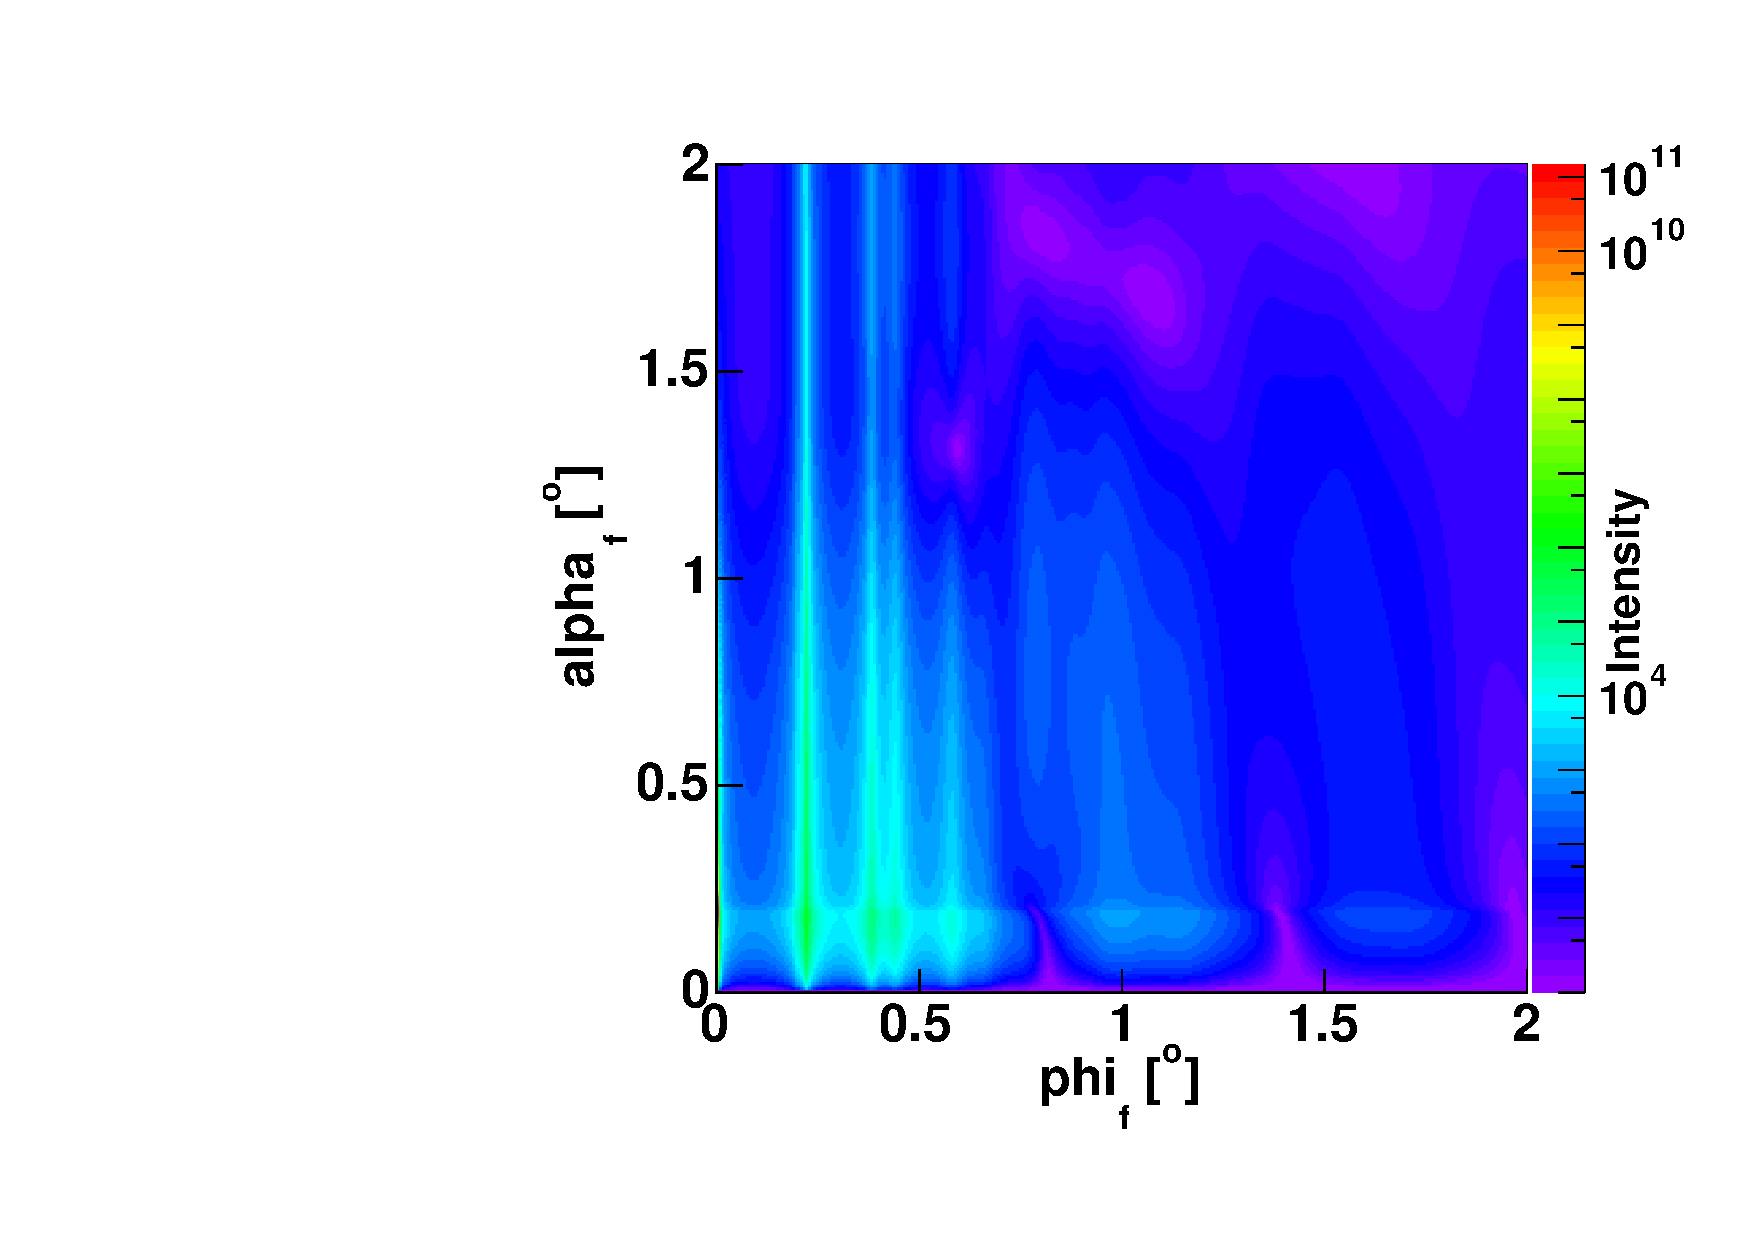
\includegraphics[angle=-90,width=0.5\textwidth]{fig/gisasmap/HSphere_2DDL.pdf}
\end{center}
\caption{Output intensity scattered from a sample made of half-spheres with 2DParacrystal interference function.}
\label{fig:2ddl}
\end{figure}

\FloatBarrier


%===============================================================================
\subsection{Summary}
%===============================================================================

\begin{table}[h]
  \footnotesize
\begin{tabular}{lll}
\hline
Function  & Parameters & Comments\\
\hline
\Code{InterferenceFunctionNone}  & None & disordered distribution \\
\hline
\Code{InterferenceFunction1DLattice} & \Code{lattice\_length} & use only with infinitely long/wide particles \\
  & $\xi=\widehat{(\v{x},\v{a})}$ & pdf=(Cauchy, Gauss or Voigt)  to be defined\\
\hline
 \Code{InterferenceFunctionRadialParaCrystal}  & peak\_distance of pdf & pdf=(Cauchy, Gauss or Voigt) to be defined \\
& damping\_length (optional) & \\
\hline
 \Code{InterferenceFunction2DLattice}  & L\_1, L\_2: lattice lengths & pdf=(Cauchy, Gauss or Voigt) to be defined\\
                        & lattice\_angle=$\widehat{(\v{a},\v{b})}$ & \\
                                                            & $\xi =\widehat{(\v{x},\v{a})}$ & \\
\hline
\Code{InterferenceFunction2DParaCrystal}  & L\_1, L\_2: lattice lengths & 2D pdf=(Cauchy, Gauss or Voigt) to be defined \\
                          & lattice\_angle=$\widehat{(\v{a},\v{b})}$ & (1 pdf per axis) \\
& $\xi=\widehat{(\v{x},\v{a})}$ & \\
& damping\_length (optional)  &  same for both axes\\
\hline
\hline
\end{tabular}
\caption{List of interference functions implemented in \BornAgain. pdf : probability distribution function, $\v{a}, \v{b}$ are the lattice base vectors, and $\v{x}$ is the axis vector perpendicular to the detector plane.}
\end{table}

\index{Particle assemblies)}%
%\fi
